\documentclass[letterpaper]{article}
\usepackage[margin=1.25in]{geometry}
\usepackage{amsmath}
\usepackage{amssymb}
\usepackage{titling}
\usepackage{graphicx}
\usepackage{caption} 
\usepackage{float}
\usepackage{subfig}
\usepackage{enumitem}
\usepackage{parskip}
\usepackage{titlesec}
\usepackage{mathtools}
\usepackage{url}

\usepackage[backend=biber,style=apa,citestyle=authoryear]{biblatex}

\addbibresource{citations.bib}

\allowdisplaybreaks
\title{
	\textbf{Politech Mathematical Group} \\ 
	\vspace{2ex} 
	Political Fatness Report
	\vspace{2ex}
}
\author{
	Darren Kong \\ 110770716
	\and 
	Hugo Mainguy \\ 111747982
	\and 
	Jeffrey Zhong \\ 112299792
	\vspace{3ex}
}
\date{March 29, 2021}

\begin{document}


\begin{titlepage}
\maketitle
\thispagestyle{empty}
\end{titlepage}

\section{Abstract}
%TODO%
% still a little rough %
The issue of fair congressional districts has long been an issue in the United States, as many criteria varying from state to state are considered in the process of creating fair districting plans. The goal of redistricting is loosely defined and the process often completed by parties with little interest in nonpartisanship. Some instances in the past have used the Polsby-Popper test as one way to calculate compactness and the test generally favors geometrically compact shapes. However, Polsby-Popper does not account for the distribution of the population within the shape and its surroundings, and as such, may unnecessarily punish non-compact districtings. The paper therefore investigates an alternate compactness measure that factors in the distribution of the population alongside the geometry of a districting, with the convex hull. Using the Automated Redistricting System, we calculate the convex hull score alongside the Polsby-Popper score for the districts of several U.S. states. Graphing the results, we examine the extrema in each quadrant to determine the attributes that most affect each measure. It may be of interest to weigh the Polsby-Popper test score and the convex hull score together for a better measure of compactness. 


\section{Introduction}

The advent of technology, especially in more recent times, has made every aspect of life “more” something. For instance, we are more connected with the Internet and instant communication across the globe than we were with letters, or printed newspapers. It may seem that this intensification of long-distance communication should make us all closer to one another. Yet, it seems that technology has also made mankind more divided, with the decentralization of news outlets or American politics. With the advent of technology, the decennial process of redistricting states with more than one congressional district has become a partisan affair. Fewer districts are competitive now than even twenty years ago such that there is less need to appeal to the other side (\cite{cook}). This has led to the increase polarization of the political forum.

It is easy to call out gerrymandering, yet, at the same time, difficult to give precise measures for it. In Vieth v. Jubelirer, ruled in 2004, the Supreme Court argued that a districting was not gerrymandered due to the lack of a measure to quantify inequality or lack of fairness (\cite{vieth}). As courts – especially the Supreme Court – often rule by precedent, this ruling has been used as an excuse to bring down some cases that made it to the highest court of the land. This has emboldened strategists to make increasingly “unfair” maps. The surge in gerrymandered districting plans is the combination of three factors that all came together at the same time: large political successes for one party, the Republicans, just before drawing districts, the sudden improvement of technology, and the increasing polarization in voting patterns.

This comes together in what could be considered a paradox: while there are ever more accurate methods to gerrymander at will, there is no mathematical standard accepted by the courts to identify the practice as of today. Furthermore, state constitutions tend to lag even further behind, because of the amount of the slow legislative process and support required to change them. Only twenty-three states require their congressional districts to be contiguous (\cite{contiguity}). While in practice, this is virtually always the case, it leaves the potential for gerrymandering in over half of the states. (Contiguity refers to the fact that any point of the district must be accessible from any other point of the district without leaving it, except for example if part of it is an island and there is a method of transportation such as a bridge or a regular ferry between both sides.) Furthermore, only eighteen states have any mention of compactness for their congressional districts. Within those eighteen states, a minority have more legal requirements. For instance, Iowa requests that districts not be oddly shaped (the state is almost a rectangle that can be split equally in four rectangles), California asks for districts not to bypass nearby large population areas for more distant populated areas, Arizona requires at least some of the districts to be competitive if feasible, and Rhode Island to represent the state fairly (\cite{contiguity}). Furthermore, there are additonal legal requirements for many state redistricting efforts to have communities of interest be in the same district (\cite{brennan}). Overall, there is a lot of leeway in what can be done by the redistricting committee. 


\section{Methodology}
To counter this, we suggest setting a standard with a definition of compactness. Compactness is something easily perceivable by humans, yet, there is no measure that satisfies human perception all the time - and we sometimes disagree among ourselves (\cite{king}).
However, a generally sensible choice is using the Polsby-Popper measure (\cite{polsbypopper}), which is given by the formula:

\[
	PP(D) = \frac{4\pi A(D)}{P(D)^2}
\]

% Need sources for these claims

Where $A(D)$ is the area of the object $D$ and $P(D)$ its perimeter. This gives us a ratio between 0 and 1. It is 0 precisely when the area is 0 ($D$ is a line or a point) and 1 when $D$ is a circle. In particular, this favors compact round objects, and opposes those with longer or jagged perimeters. Both of these are important, and the measure has been used in real life, for instance with Arizona’s redistricting in 2000 (\cite{moncrief}). It is noteworthy that several states use different measures, particularly in the West, where more attention is paid to fairness.

Other measures are used in different states: for instance, in Colorado, the districts should minimize the total perimeter. States like California and Michigan instead focus on dispersion rather than contorted boundaries, as Moncrief points out. 

It becomes clear that the Polsby-Popper measure only takes into consideration the geometric compactness or fatness of the redistricting shape. Many measures of geometric fatness have used a generalized ratio of what is inside and outside of a shape. For example, a type of geometric fatness would be the ratio of the area of a inscribed circle over the area of the bounding circle (\cite{fatness}). We had built upon that idea of fatness by utilizing the convex hull of a shape rather than the inscribed and bounding circles. Additionally, more suitable measure for compactness would also take into consideration the population requirement of the districtings. All congressional districtings have to be equal in population at the time of the redistricting. For example, a congressional district may seem to be shaped oddly but that is only due to the legal requirement for equal population size (\cite{westberryVsanders}). However, there are legal precedents, (\cite{sandiego}) and (\cite{california}), that say a district cannot be oddly shaped for the purpose of equal populations if the odd shape bypasses a nearby populaton center to reach population centers further away. That is one of the features that may indicate gerrymandering.

Here we will propose an alternative to the Polsby-Popper that will be referred to as the Convex Hull measure. To calculate this measure, we use the following formula:

\[
	\frac{POP(D)}{POP(CH(D))}
\]

Where $D$ represents the district $D$, $CH(D)$ is the convex hull that contains $D$, and $POP(D)$ is the population in $D$. This measure utilizes precincts as the base level of a population cluster. Since the convex hull cuts through some precincts, in those cases, the proportion of the area of the precinct in the convex hull is used to estimate the population of the part of the precinct inside of the convex hull, yielding good approximations. Since precincts form districts, we do not need to apply any ratio other than 1 for the population inside the district borders. Furthermore, this measure only takes into account the population that is inside the state, as the population outside of the state but inside the convex hull should not influence the districts. Once again, a perfect score of 1 comes when the district is its convex hull, and a score approaches 0 when the convex hull encompasses many populous precincts, large areas of land, or a combination of both outside of the district's borders.

%[We should probably include the code for the two measures here, if anyone feels like adding it. Actually, maybe after each measure, whatever is better.]%

Since these two measures are different, it is interesting to compare them to see when they are similar and when they differ, explain why that is the case, and conclude whether those districts are gerrymandered or not. We used a total of nine states: New York, Pennsylvania, Virginia, North Carolina, Georgia, Texas, Utah, Oregon, and Ohio. Using the current congressional districts, here are the data points found (Pennsylvania and North Carolina maps are from 2016).

\section{Results}

\begin{figure}[H]
	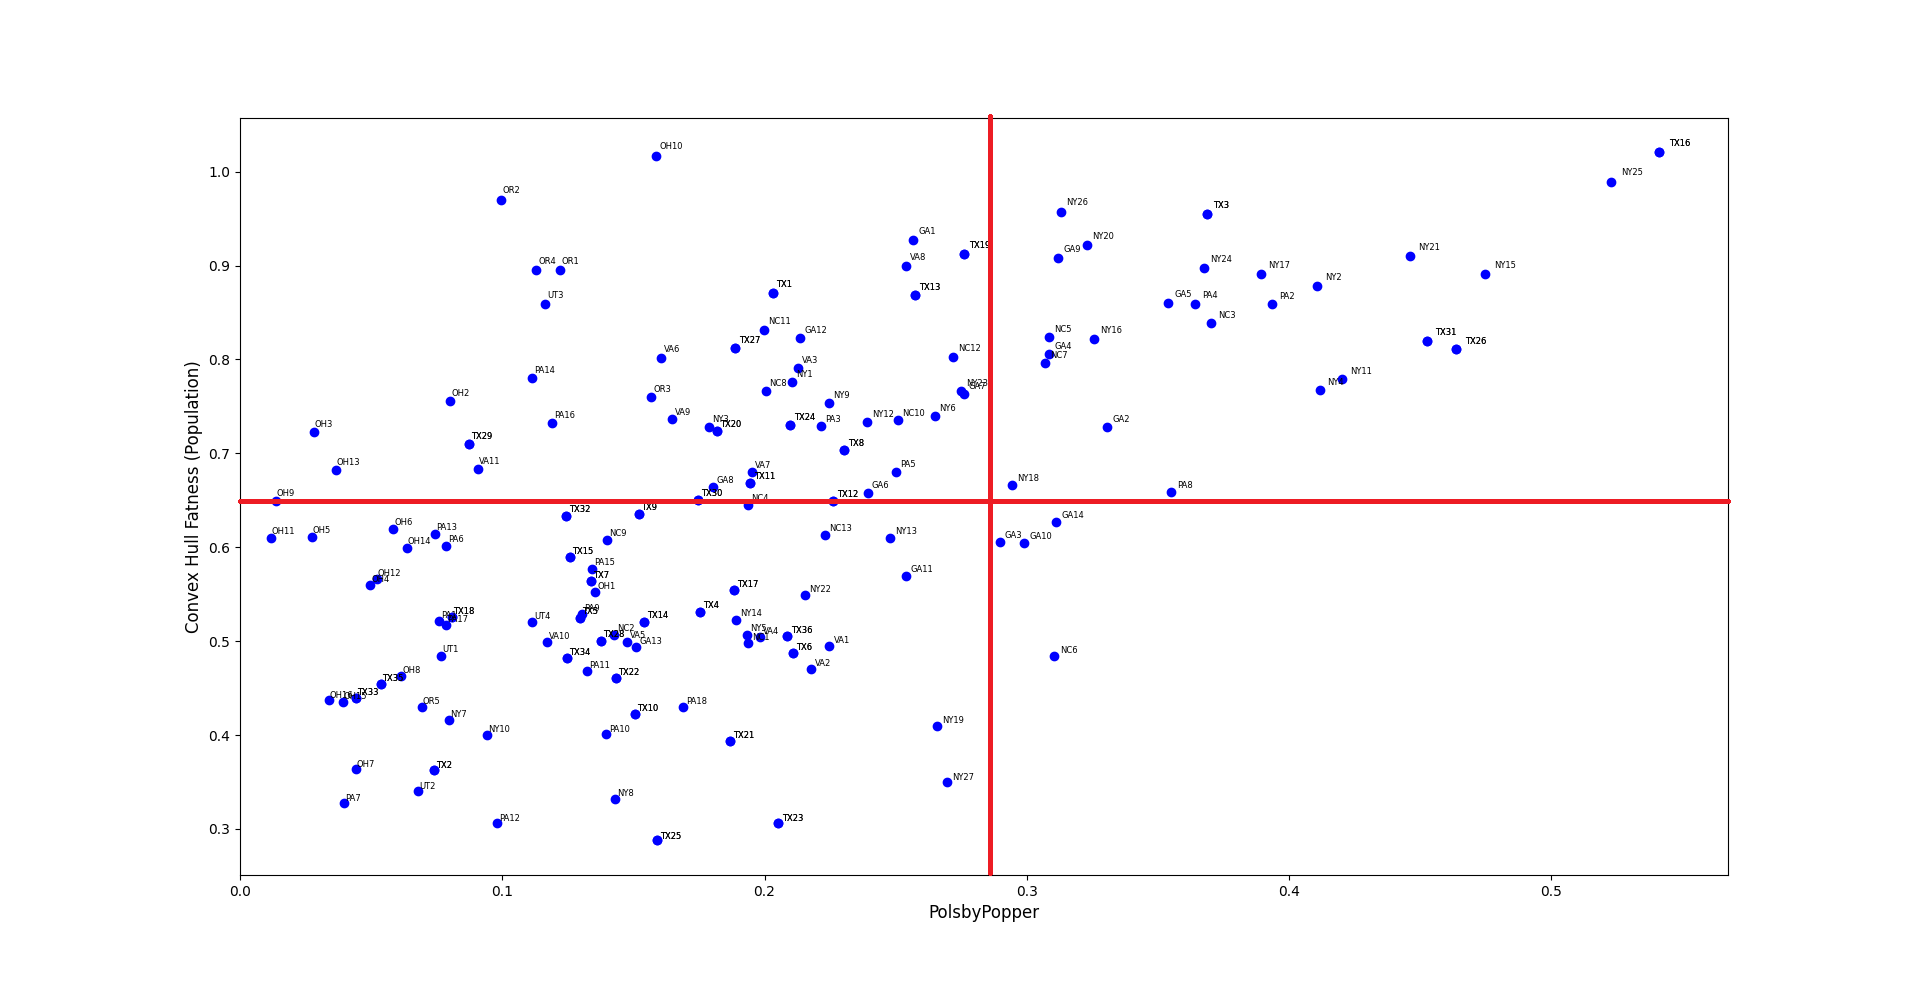
\includegraphics[width=\linewidth]{./figures/convexHullPopulationFatnessVPP2Edited.png}
	\caption{Plot of Population Fatness v. PolsbyPopper}
	\label{fig:datapoints}
\end{figure}

\section{Analysis}
From the results, we can compare each district's Fatness score with its Polsby-Popper score. There is a slight positive correlation between the Fatness and PolsbyPopper scores.
To help easily identify the location of specific districts, we will split the graph into four quadrants. The quadrants are to be referred from 1 to 4 starting from the top right in a counterclockwise fashion. We do this to identify extremeties in each of the district scores to see in what cases these two scores may differ wildly.

\subsection{Low Fatness and High Polsby Popper}
We will make a quick remark on the fourth quadrant. This is the quadrant where we would have a low Fatness score and a high Polsby Popper score. The point of this quadrant is to find the districts which Polsby Popper identifies as a good district but Fatness identifies as a bad district. In essence, if we use Polsby Popper to categorize good and bad districts, this quadrant would represent the false positives. It is mostly empty except for the inclusion of North Carolina's 6th congressional district (the one in use for the 2016 and 2018 elections).

\begin{figure}[H]
	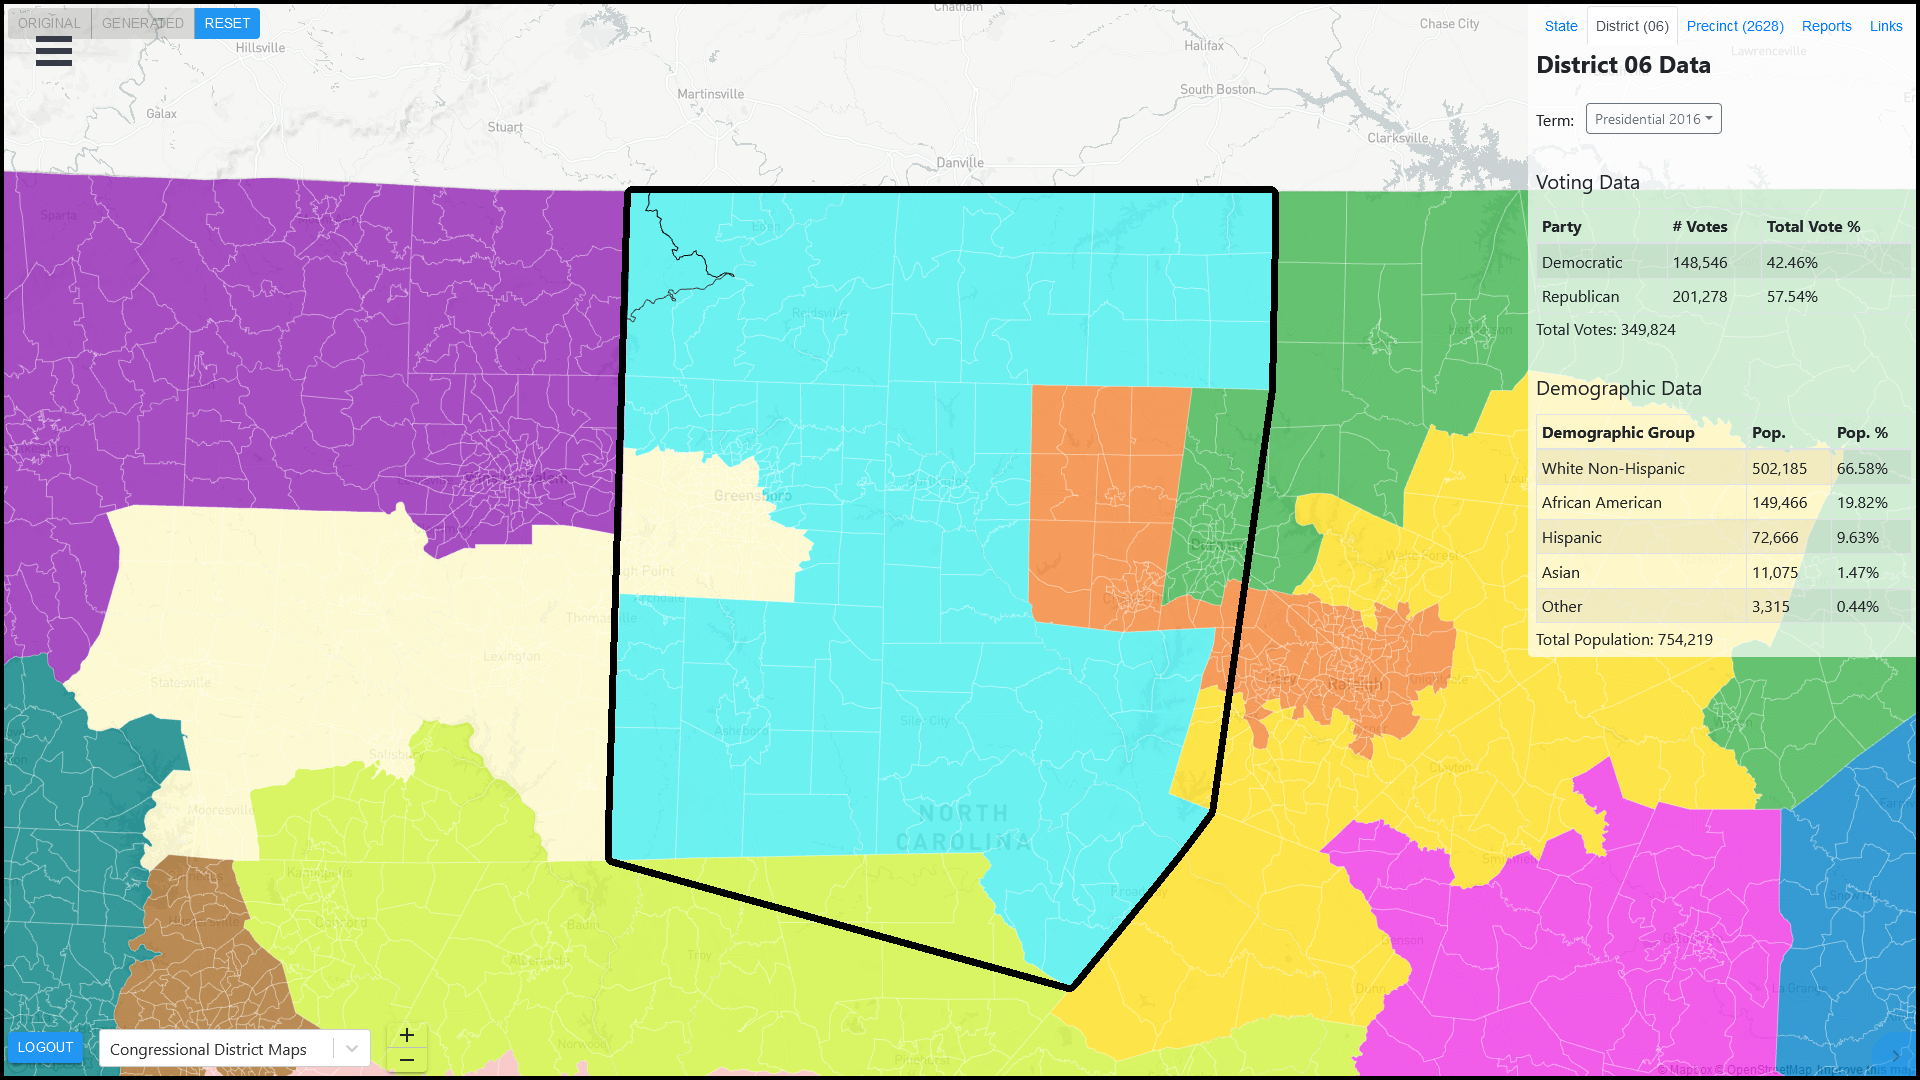
\includegraphics[width=\linewidth]{./figures/NC-06-ConvexHull.png}
	\caption{NC-06 Convex Hull}
	\label{fig:nc06convexHull}
\end{figure}

This district is actually near average on the Fatness score and PolsbyPopper score. It does seem to be an average district since it leaves the square shape near Greensboro to include the city of Winston-Salem. The extrusion into Winston-Salem seems to be jarring due to the initial square shape. Furthermore, the two areas excluded both slightly west and east of the center of the district are heavily Democract, which allows the district to elect a Republican by a rather small margin. The area around Durham is then joined with Raleigh for a strongly Democract district, while the Democrat votes west of NC-06 are themselves added into another Republican district. The former Representative of NC-06 chose not to run again and has been replaced by a Democratic challenger in 2020, showing some of the consequences of switching to a fairer map raising the number of Democrat representatives in the state from three to five.

\subsection{High Fatness and High Polsby Popper}
We will now turn our attention onto the districts in the first quadrant, specifically NY-25, NY-15, and TX-16. The district scores for both the Fatness and Polsby-Popper measures are both high for these districts. It is rather easy to tell why.

\begin{figure}[H]
	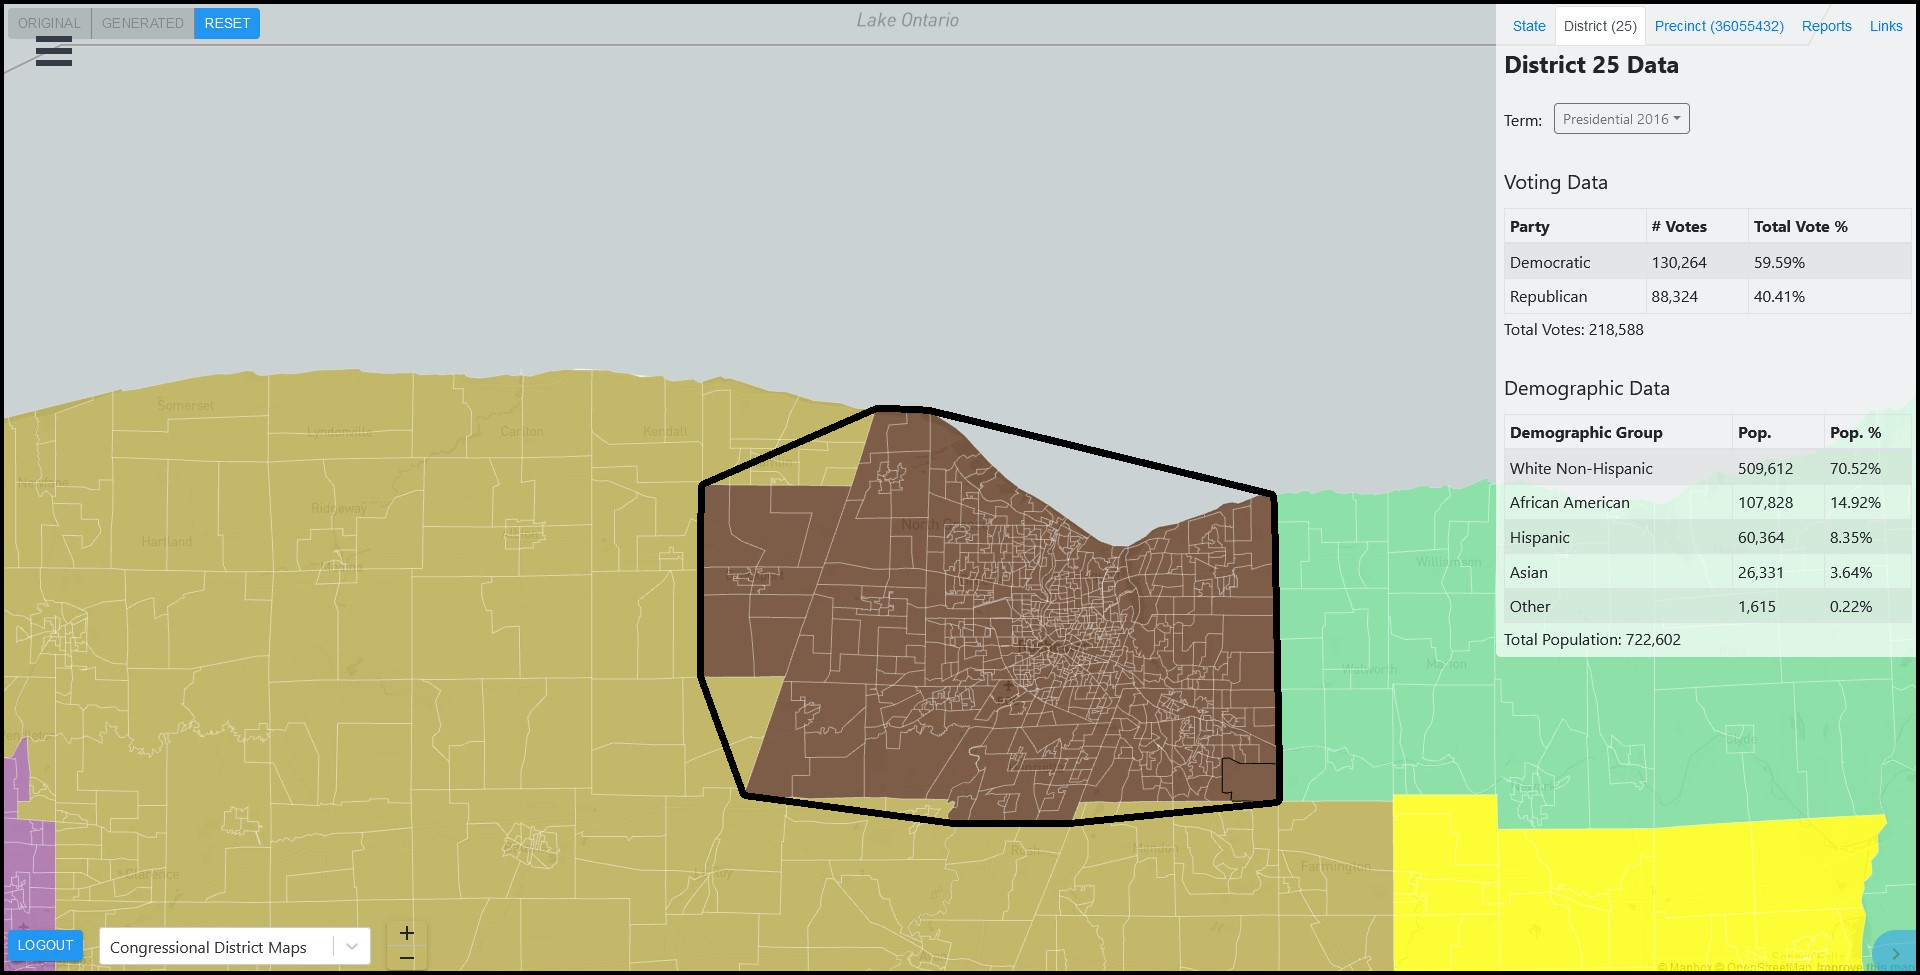
\includegraphics[width=\linewidth]{./figures/NY-25-ConvexHull.png}
	\caption{NY-25 Convex Hull}
	\label{fig:ny25convexHull}
\end{figure}

\begin{figure}[H]
	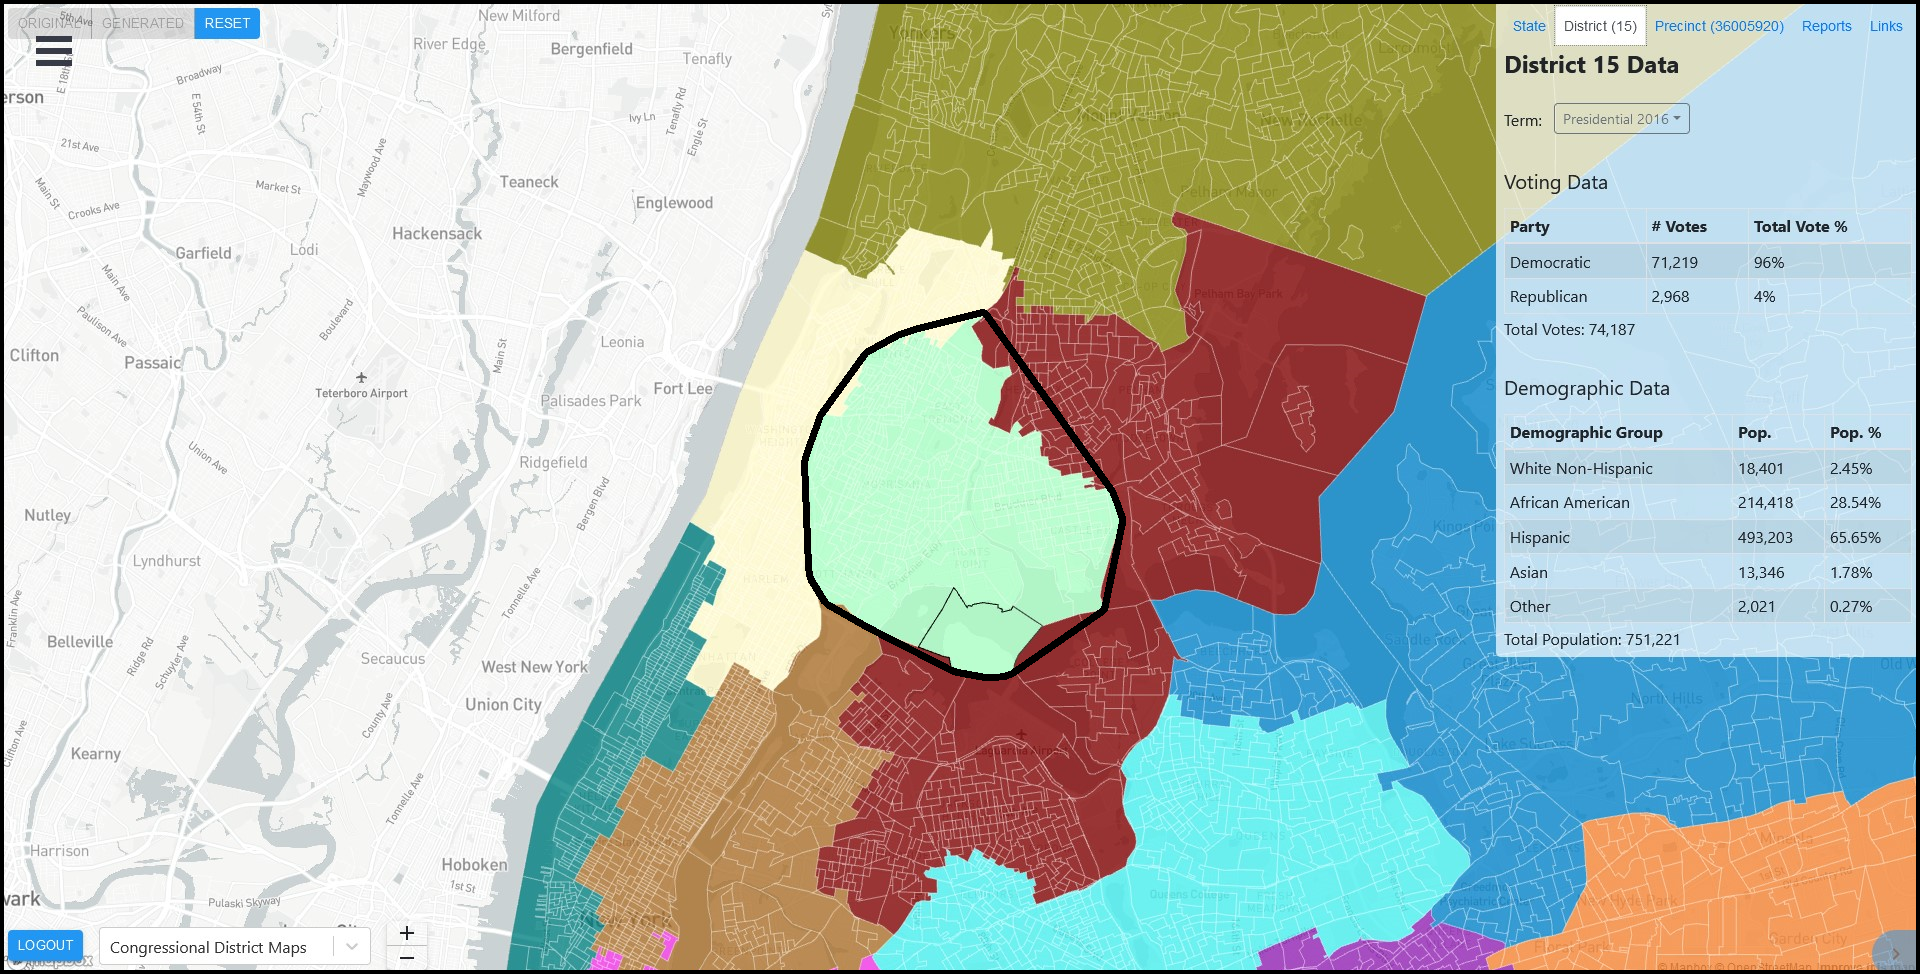
\includegraphics[width=\linewidth]{./figures/NY-15-ConvexHull.png}
	\caption{NY-15 Convex Hull}
	\label{fig:ny15convexHull}
\end{figure}

\begin{figure}[H]
	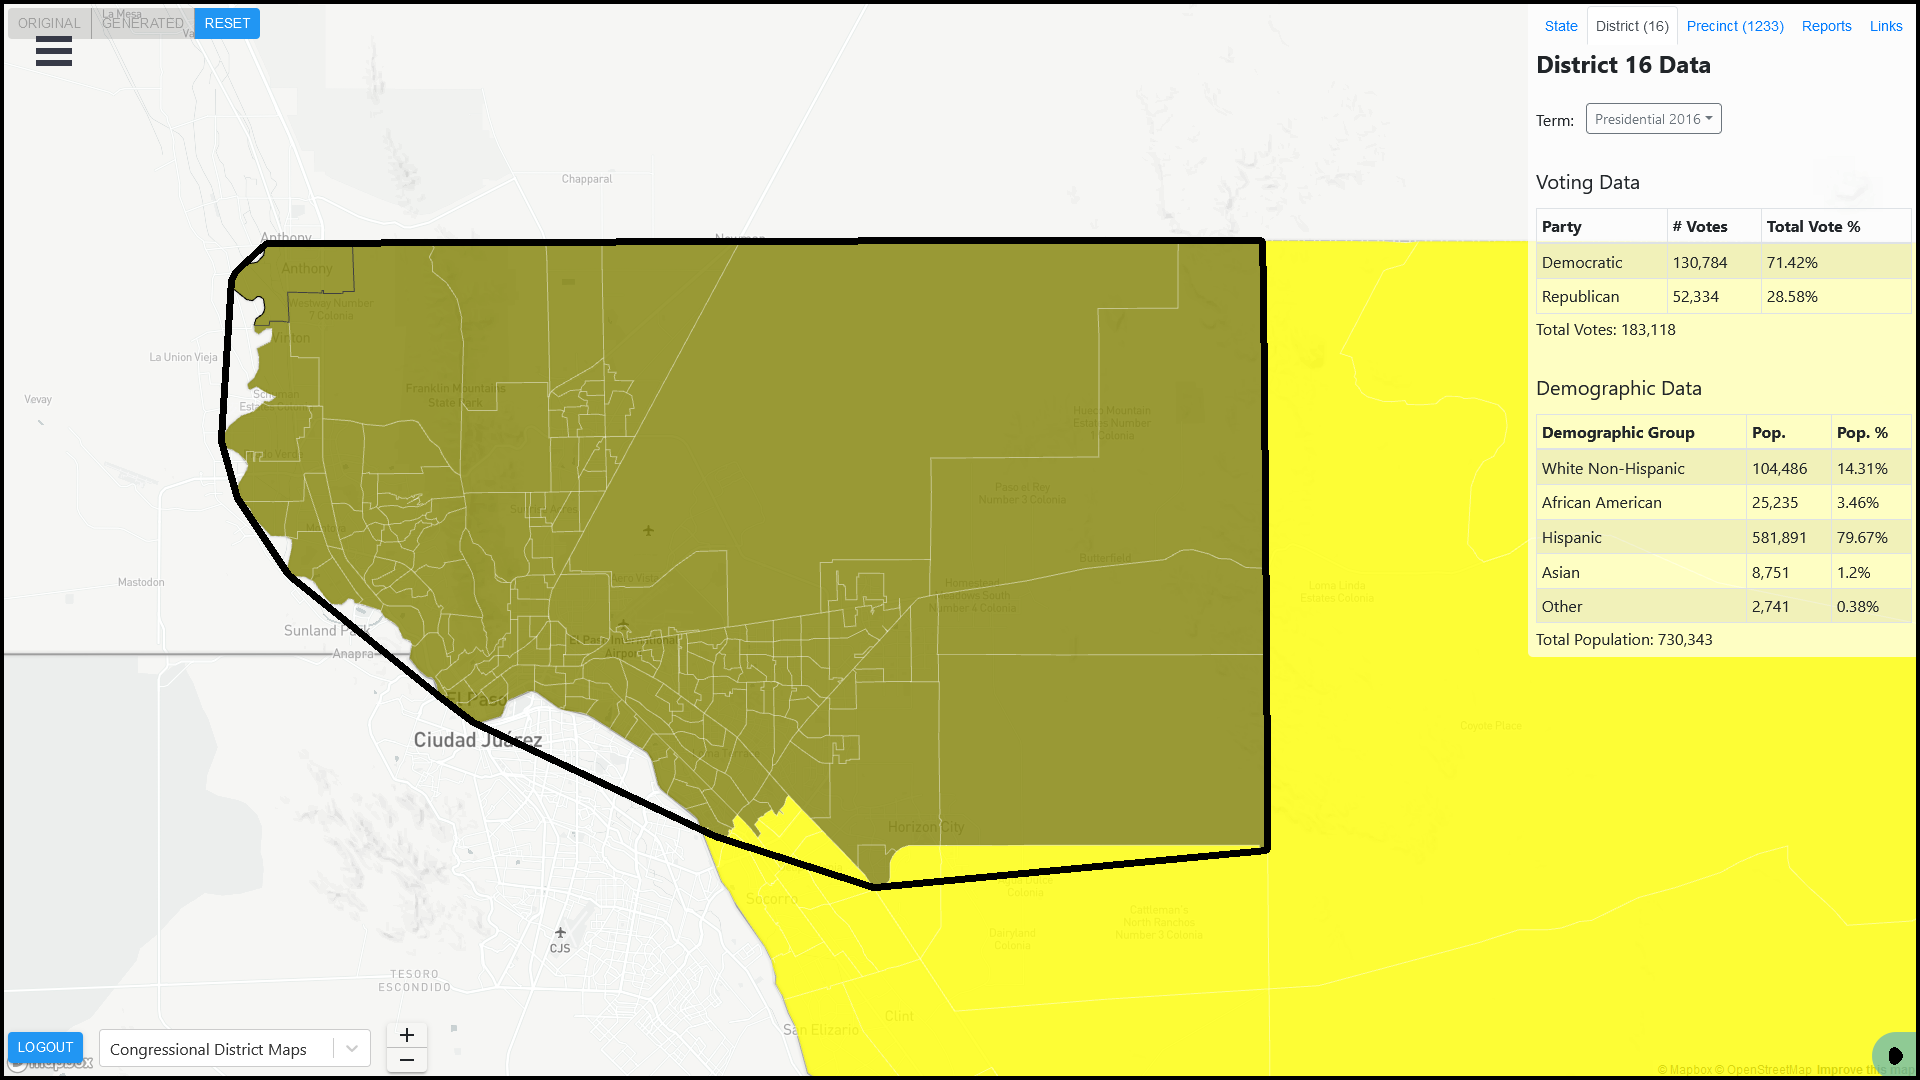
\includegraphics[width=\linewidth]{./figures/TX-16-ConvexHull.png}
	\caption{TX-16 Convex Hull}
	\label{fig:tx16convexHull}
\end{figure}

These districts are all centered around a major population hub. NY-25 is centered on Rochester, NY-15 is centered on the Bronx, and TX-16 is centered on El Paso. These districts geometrically all look compact and we believe that no one would considered them abnormal in any sense. This explains the high Polsby-Popper score and also partially explains the high Fatness score. 

Specifically for the example of TX-16 which takes advantage of being small and densely populated with sparsely populated districts and state/country borders around, along with straight, perpendicular borders for most of its contour. It is a very Democratic area surrounded by moderately Republican areas, but it forms a coherent district encompassing one city and its direct surroundings, and contains all but the southernmost part of El Paso County, making it a very reasonable district. It is a similar story for the other districts.

\begin{figure}[H]
	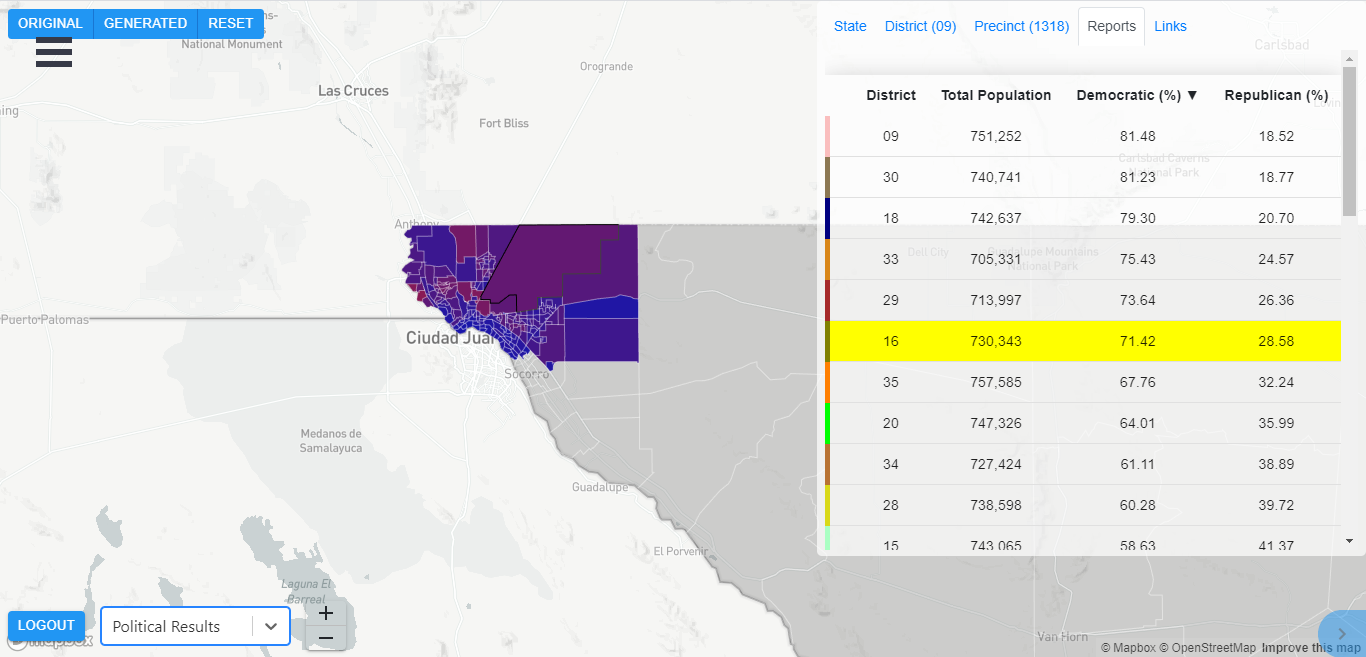
\includegraphics[width=\linewidth]{./figures/TX-16.png}
	\caption{TX-16}
	\label{fig:tx16border}
\end{figure}

\begin{figure}[H]
	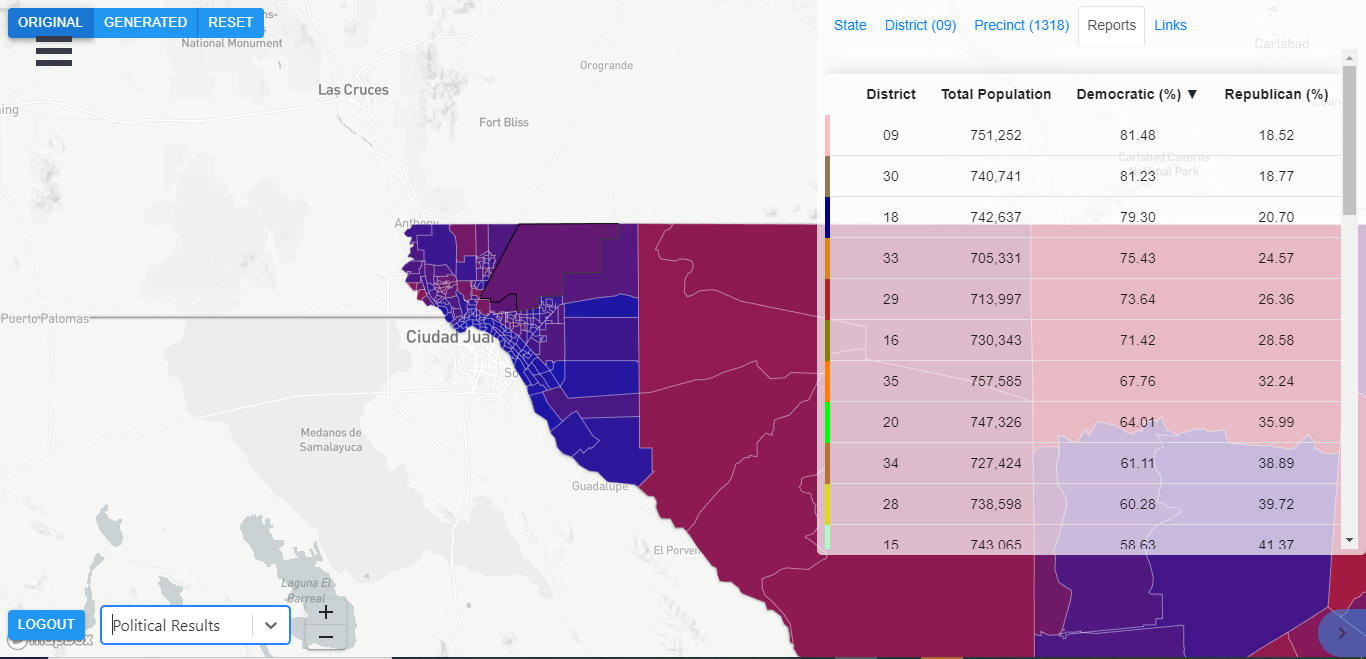
\includegraphics[width=\linewidth]{./figures/TX-16-SurroundingArea.png}
	\caption{TX-16 Political Results}
	\label{fig:tx16political}
\end{figure}

\subsection{Low Fatness and Low Polsby Popper}
We can now skip ahead to the third quadrant. These are the districts often pointed out by opponents of gerrymandering as being “bad”, failing most standard measures for compactness.

\begin{figure}[H]
	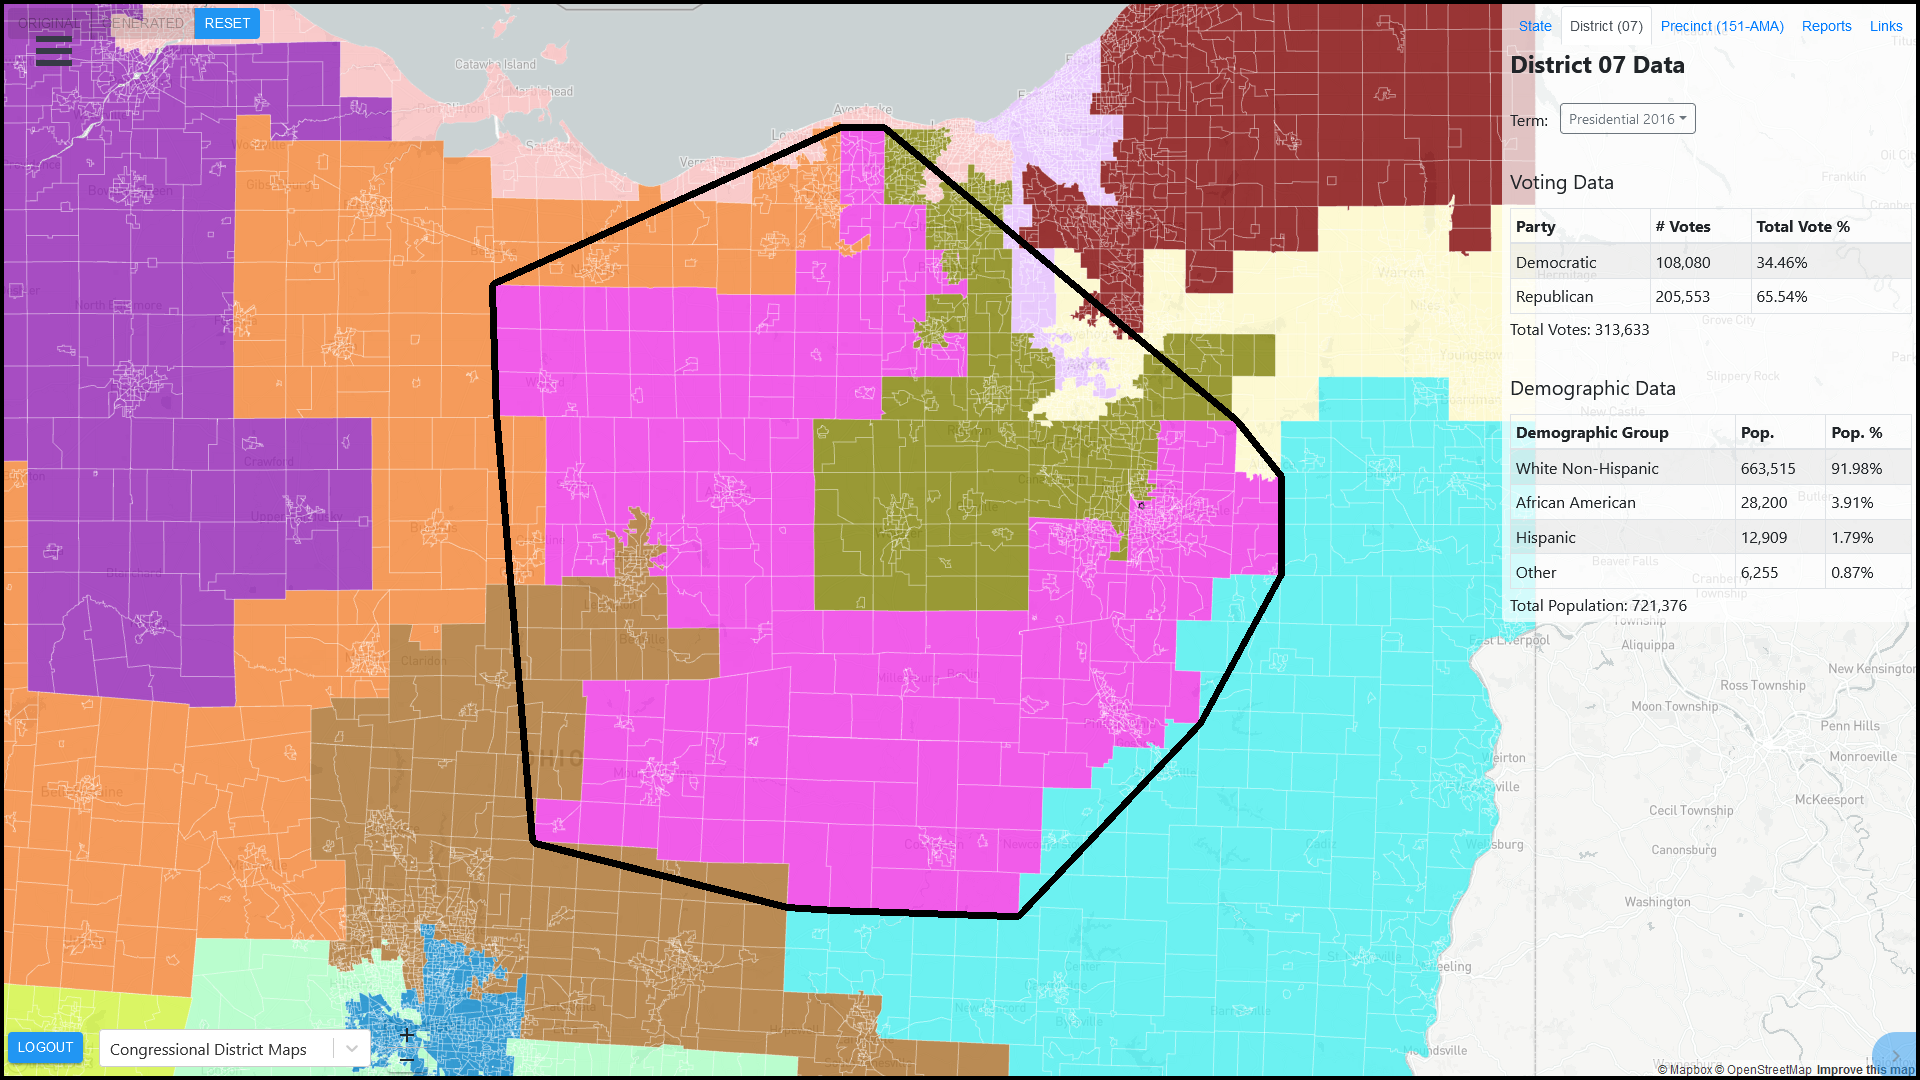
\includegraphics[width=\linewidth]{./figures/OH-07-ConvexHull.png}
	\caption{OH-07 Convex Hull}
	\label{fig:oh07ch}
\end{figure}
Ohio's 7th congressional disrict is one of the most oddly shaped districts we can find. It has a low PolsbyPopper due to low area and high border length of the district. The Fatness score is low as well due to large swaths of populations that the district bypasses but the convex hull includes. For example, the convex hull of this district would include the major city of Akron and Mansfield. From the shape of the district itself, it is deliberately avoiding these two cities. Instead of including the two cities that are near its center, the district undoubtly bypasses them and reaches for the lakeside area of Avon. This is a small Republican area between the Democratic majority cities of Cleveland and Lorain.

\begin{figure}[H]
	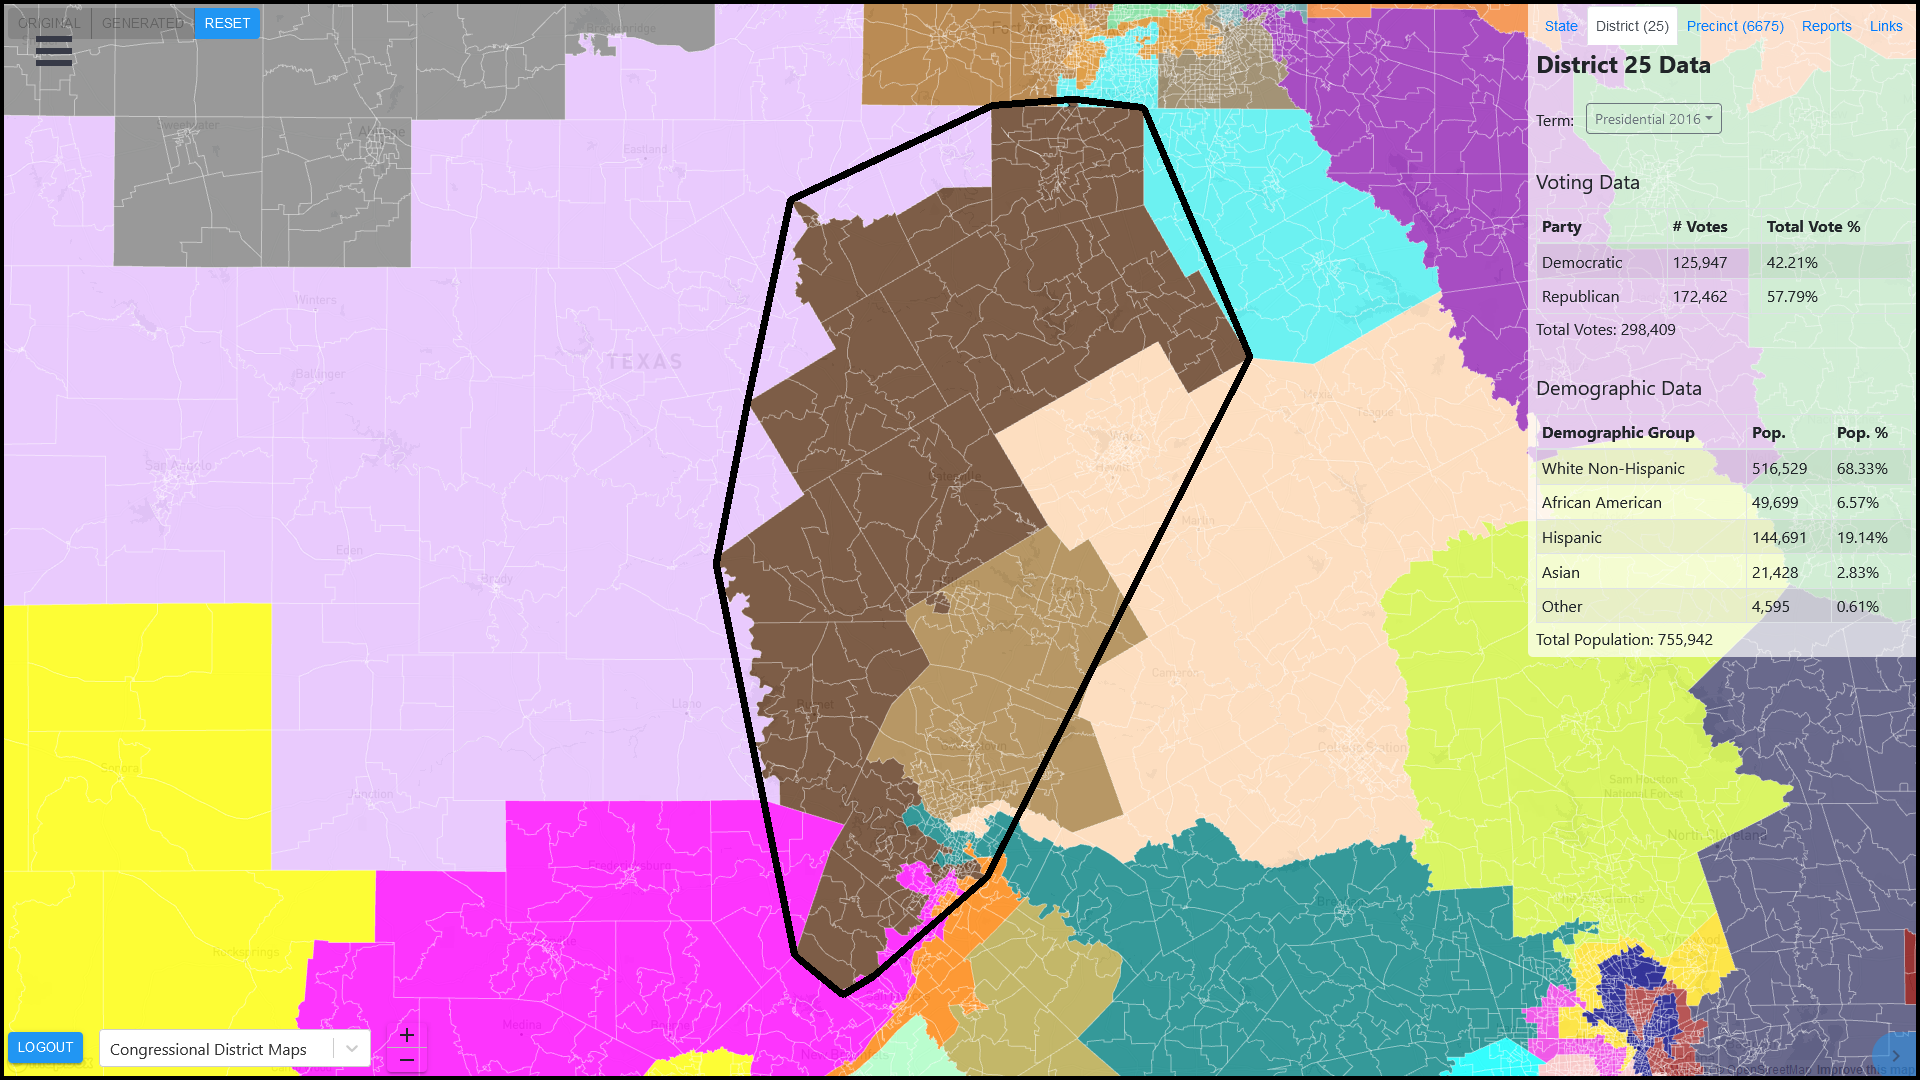
\includegraphics[width=\linewidth]{./figures/TX-25-ConvexHull.png}
	\caption{TX-25 Convex Hull}
	\label{fig:tx25ch}
\end{figure}

Another district to focus on is Texas' 25th congressional district. Here we see PolsbyPopper punish the district due to its jagged border in the east and its longer shape. The jagged edges are formed from following the rivers that feed into and leave Lake Buchanan. Furthermore, the low Fatness is primarily due to the convex hull including the city of Waco, Temple and Austin. Specifically, the shape of the district intrudes into Austin. This may have been an attempt at cracking the Democrat majority in the Austin area. The district could have been reformed instead to include Waco rather than an intrusion into Austin. Basically, the district should not have extended as south as it did and should have expanded horizontally rather than vertically.

\begin{figure}[H]
	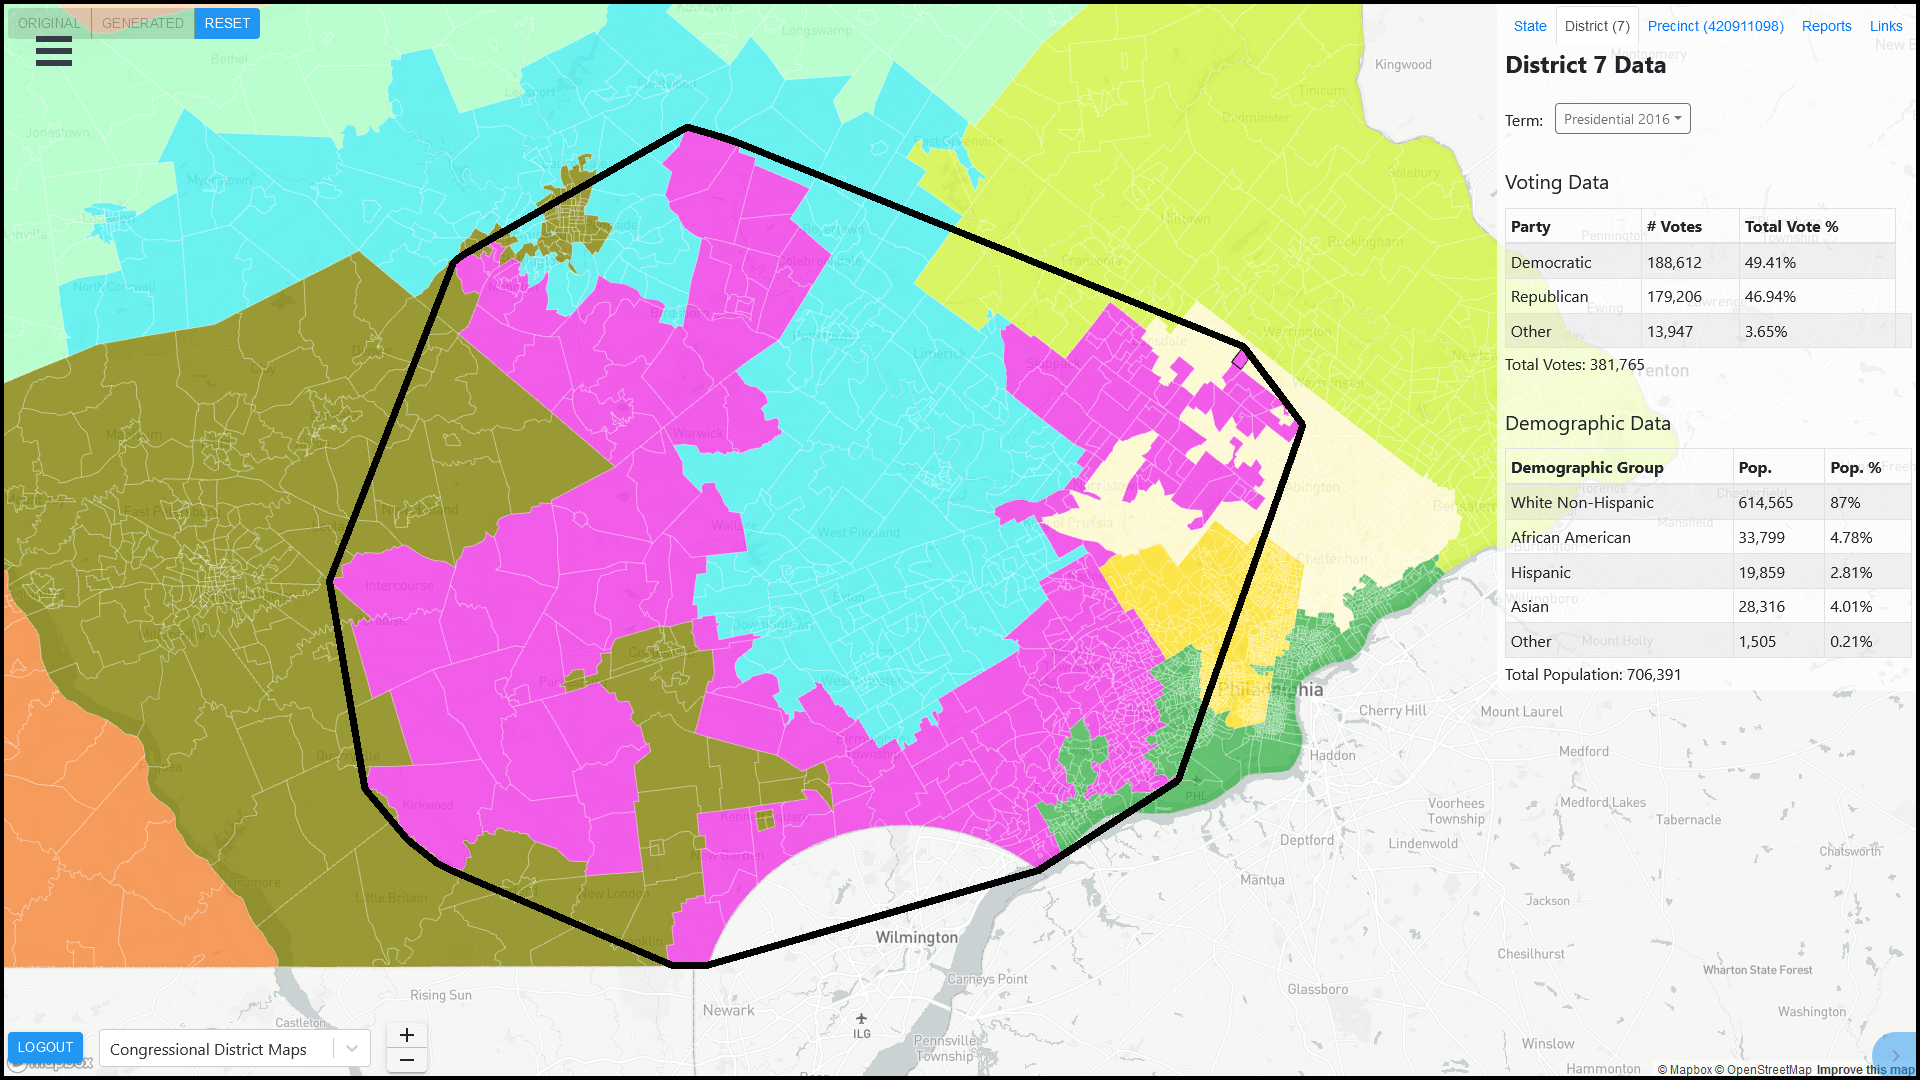
\includegraphics[width=\linewidth]{./figures/PA-07-ConvexHull.png}
	\caption{PA-07 Convex Hull}
	\label{fig:pa07ch}
\end{figure}

\begin{figure}[H]
	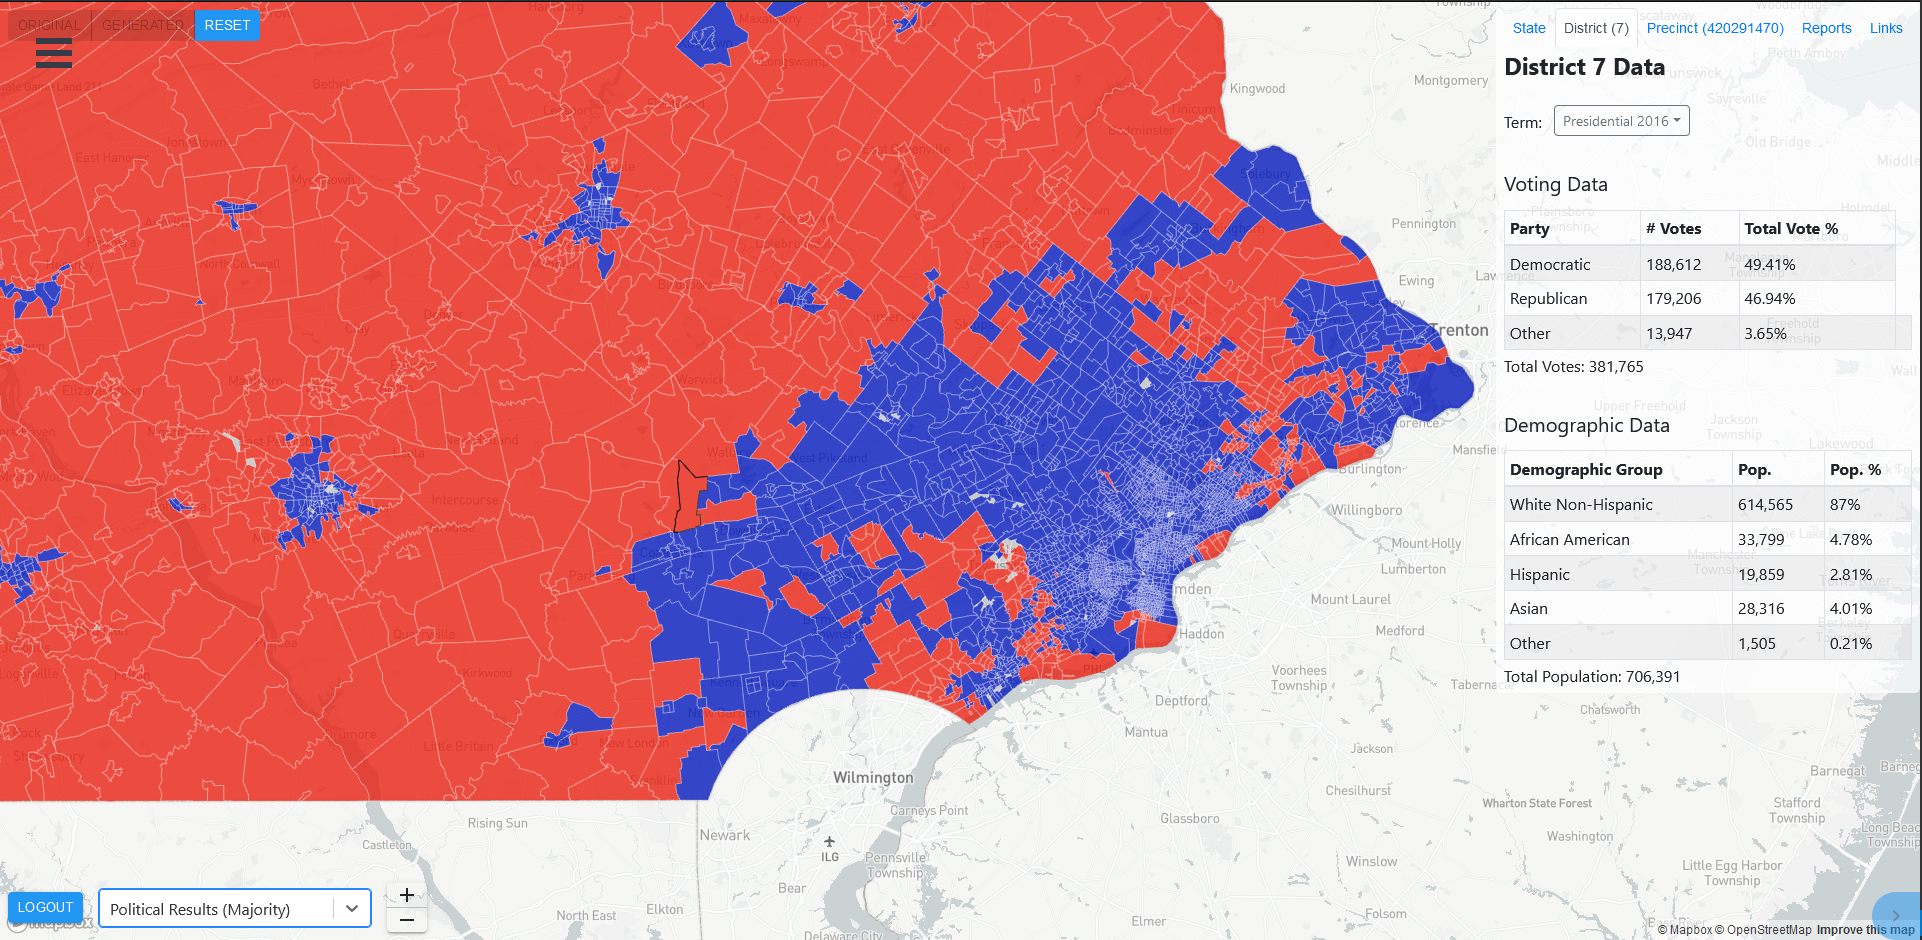
\includegraphics[width=\linewidth]{./figures/PA-07-PoliticalResults.png}
	\caption{PA-07 Political Results}
	\label{fig:pa07pr}
\end{figure}

Finally, one of the worst cases for both Polsby-Popper and Fatness is Pennsylvania's 7th congressional district. As you can see, it avoids the area containing West Pikeland that is just west of Philidelpia. If we take a look at the political results of the map, it seems to avoid the mostly Democractic majority precincts in that area. Furthermore, it seems to take the more Republican precincts to make the district more competitive for Republicans. Just as in North Carolina, this plan is no longer in use, and the change has been reflected in the political composition of Pennsylvania's congressional delegation.

\subsection{High Fatness and Low Polsby Popper}
We now move onto the extremeties in the second quadrant. The second quadrant obiouvsly contains the districts that obtained high Fatness scores but low Polsby-Popper ones. This is what would constitute a false negative categorization of districts for Polsby-Popper. The focus will be on OH-10, OR-02, OR-04, OR-01, and UT-03 as these two districts had the highest Fatness score.

\begin{figure}[H]
	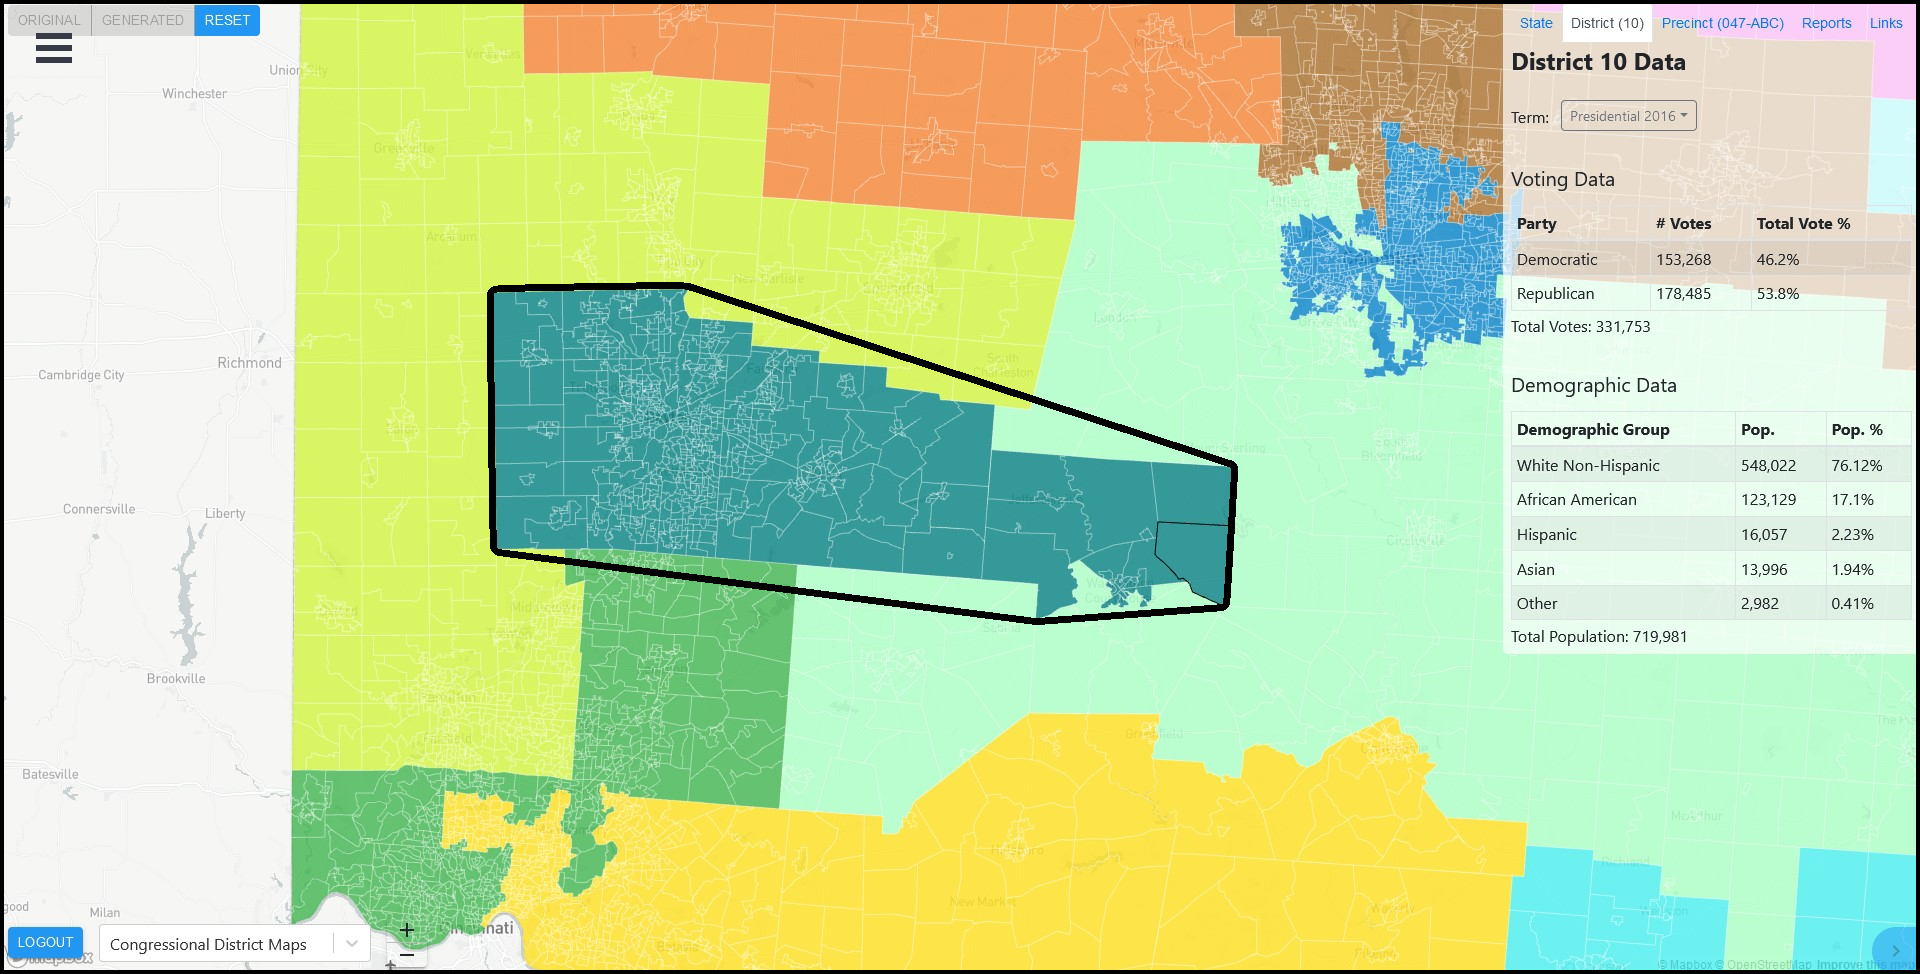
\includegraphics[width=\linewidth]{./figures/OH-10-ConvexHull.png}
	\caption{OH-10 Convex Hull}
	\label{fig:oh10convexHull}
\end{figure}

For OH-10, the Polsby-Popper measure rated this district rather low due to its long rectangle shape. Obviously, with the convex hull fatness, the score is higher as the only major difference is the removal the staircase shaped northern border of the district. Looking at the district geometrically, by itself, it would be hard to justify malicious intent.

\begin{figure}[H]
	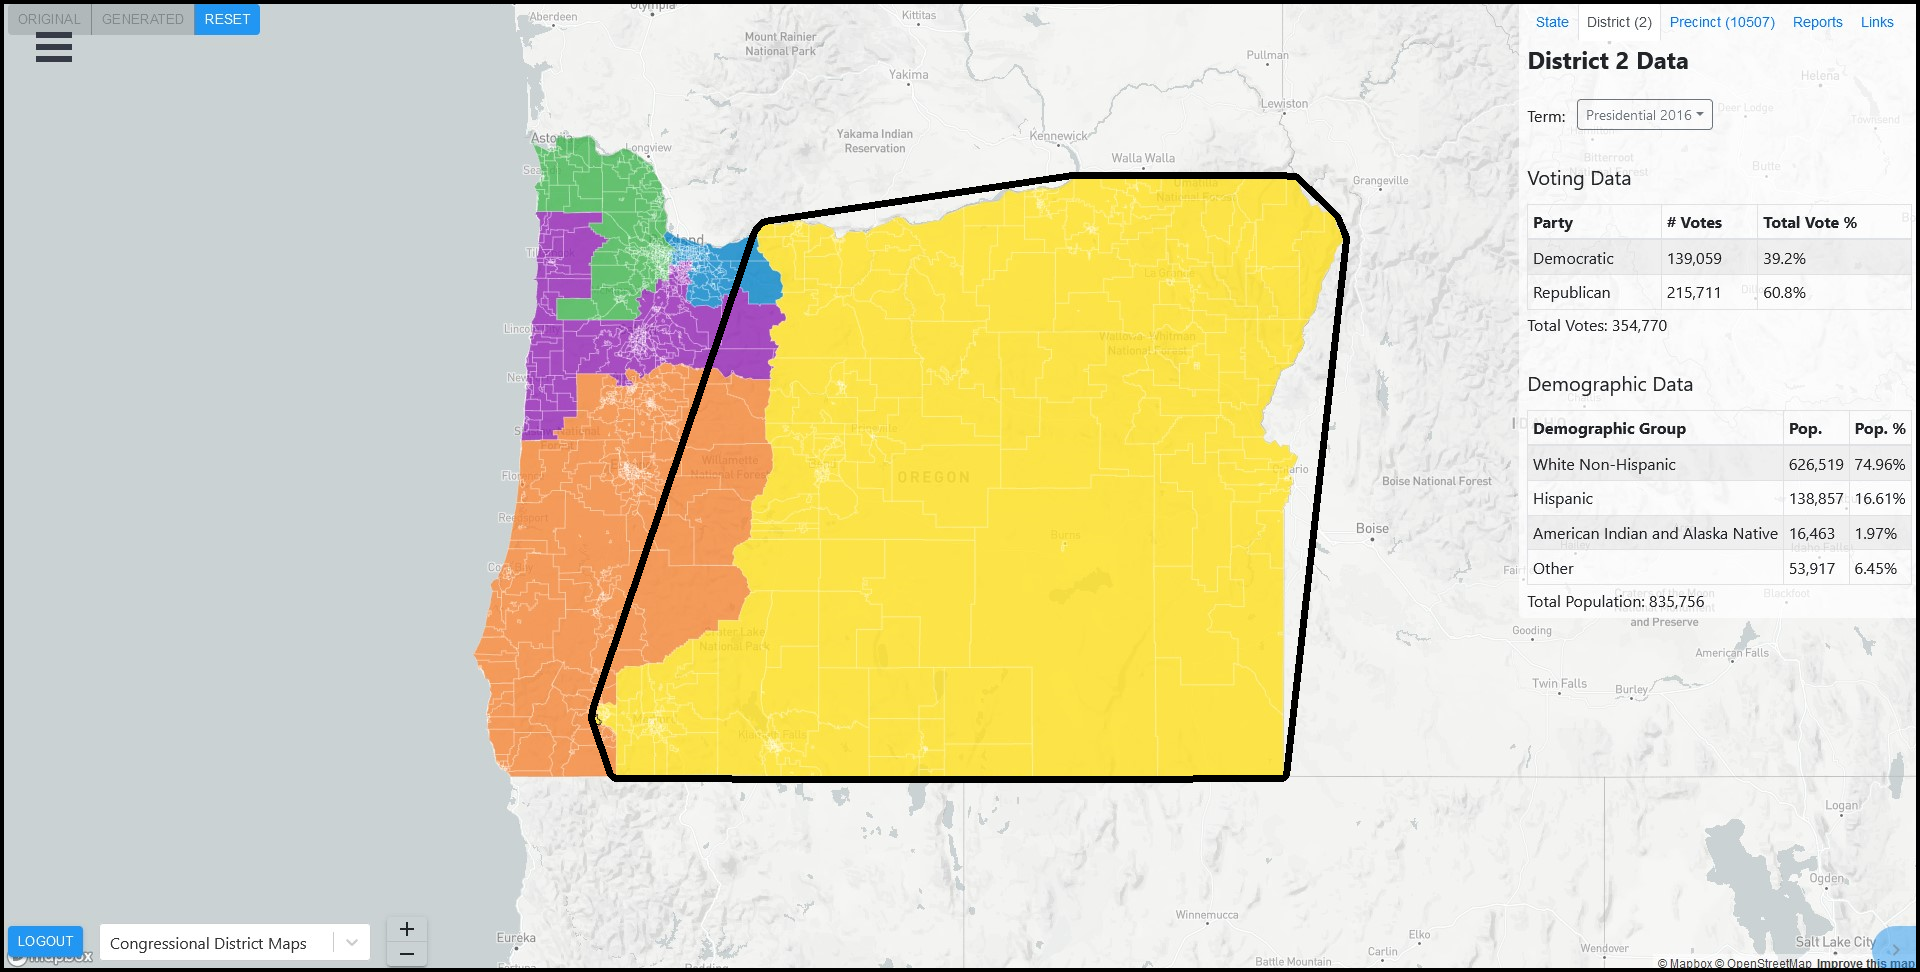
\includegraphics[width=\linewidth]{./figures/OR-02-ConvexHull.png}
	\caption{OR-02 Convex Hull}
	\label{fig:or02convexHull}
\end{figure}

A similar case can be made for OR-02. Its Polsby-Popper score was low, landing it in the left half the plot. However, it is also situated comfortable in the second quadrant where the Fatness score is high. We believe that this is a more accurate measure of the compactness of this district. There are some theories to explain the low Polsby-Popper score. If one looks closely at the border of the district, specifically the western and northern half, it is made up of jagged edges. The jagged edges constitute the district following a border represented by rivers to the north and northeast. The western portion is simply following the precincts that have the jagged edges. The many jagged edges increase the perimeter portion of the Polsby-Popper measure, therby resulting in a low score for this district. The convex hull measure is not effected as much by the jagged edges as it would change little in terms of the population that is included. Furthermore, the jagged edges are borders to the Willamette National Forest which would obviously be have a low population density even if it is included.

\begin{figure}[H]
	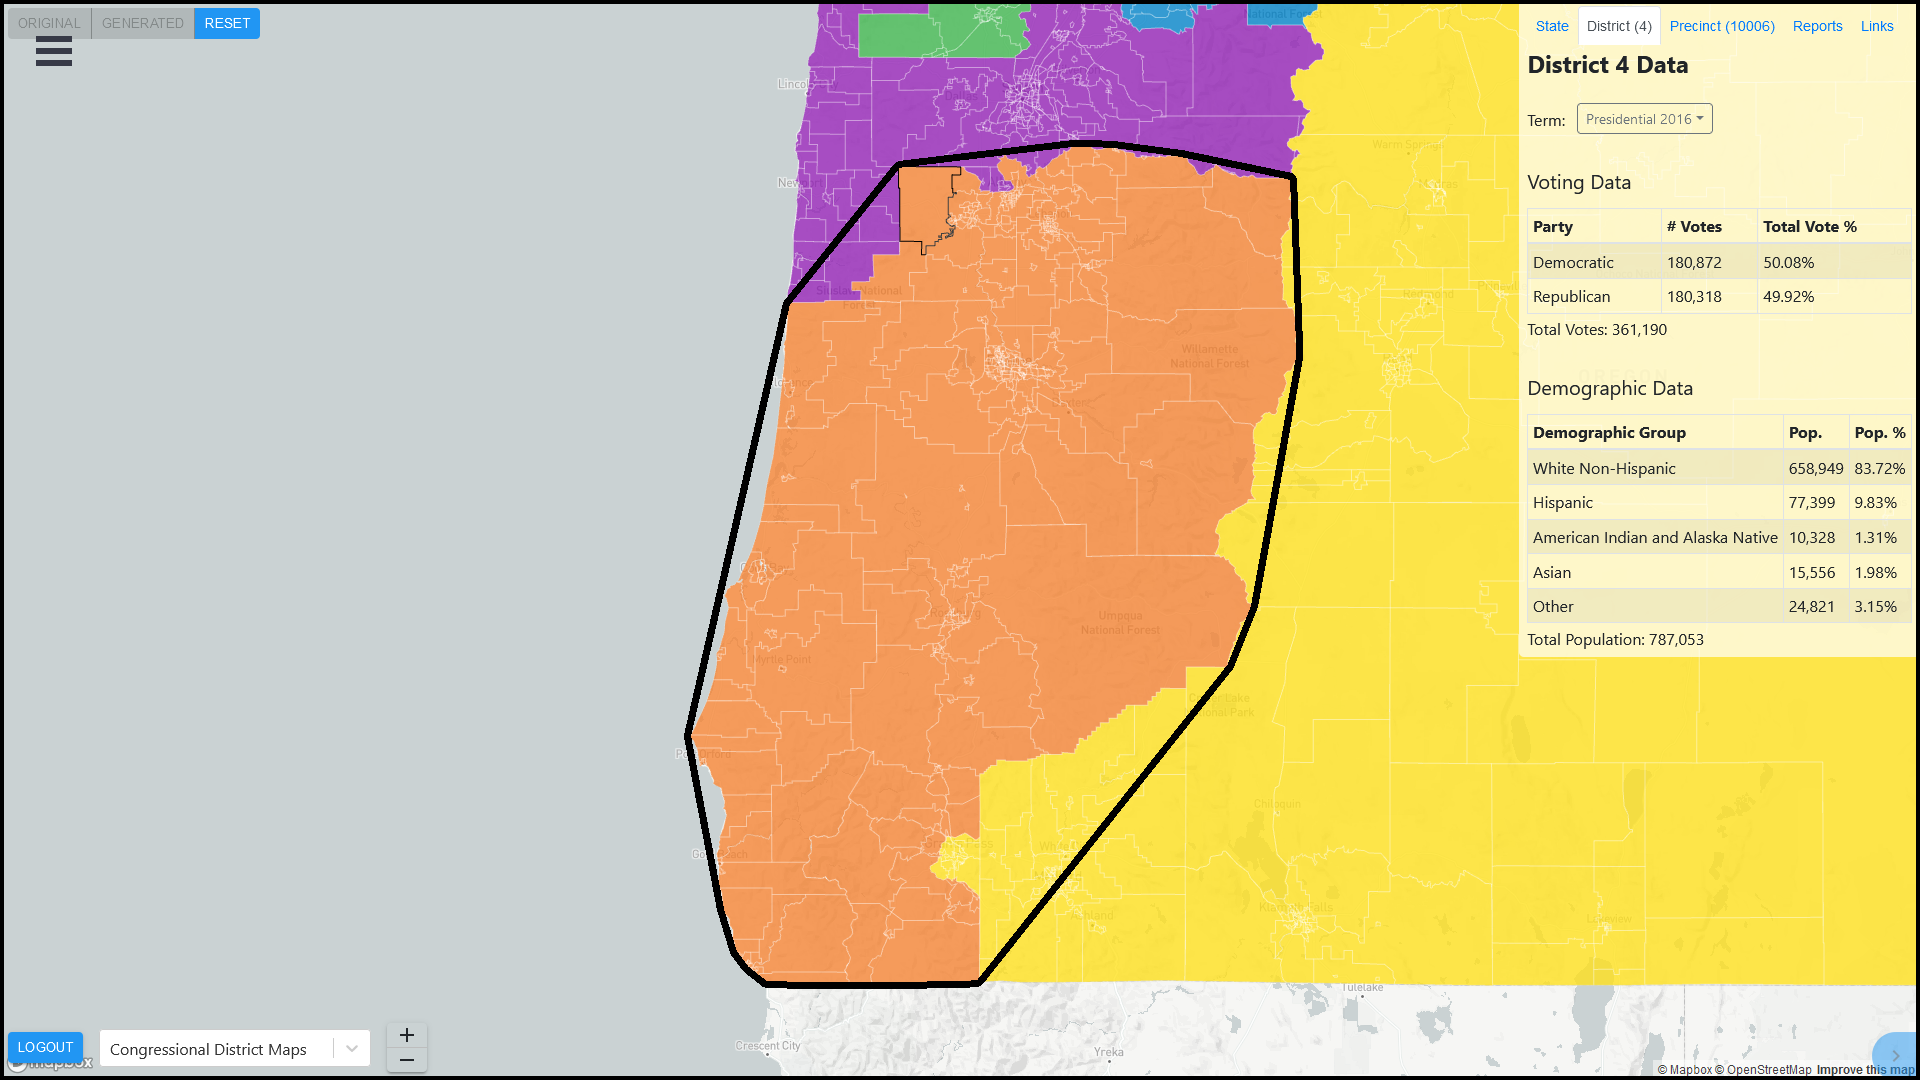
\includegraphics[width=\linewidth]{./figures/OR-04-ConvexHull.png}
	\caption{Oregon District 04}
	\label{fig:or04ch}
\end{figure}

\begin{figure}[H]
	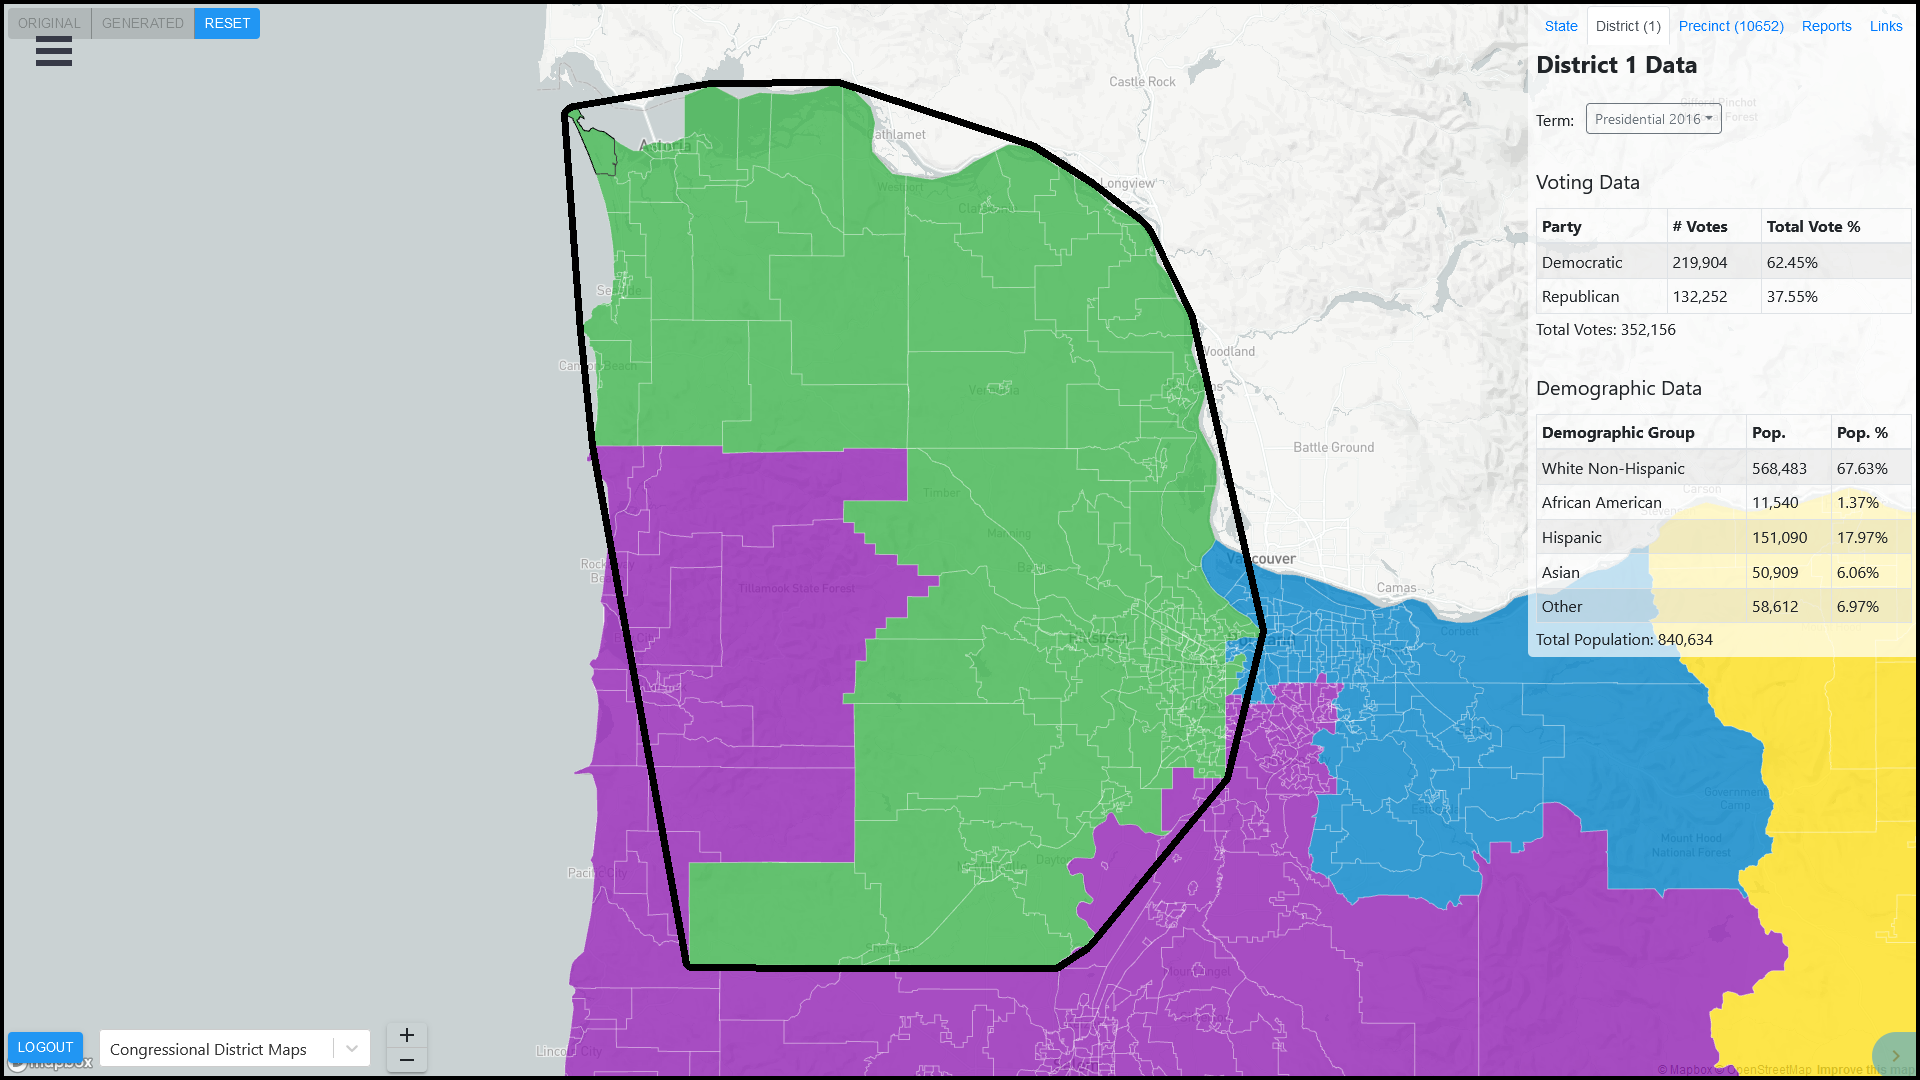
\includegraphics[width=\linewidth]{./figures/OR-01-ConvexHull.png}
	\caption{Oregon District 01}
	\label{fig:or01ch}
\end{figure}

\begin{figure}[H]
	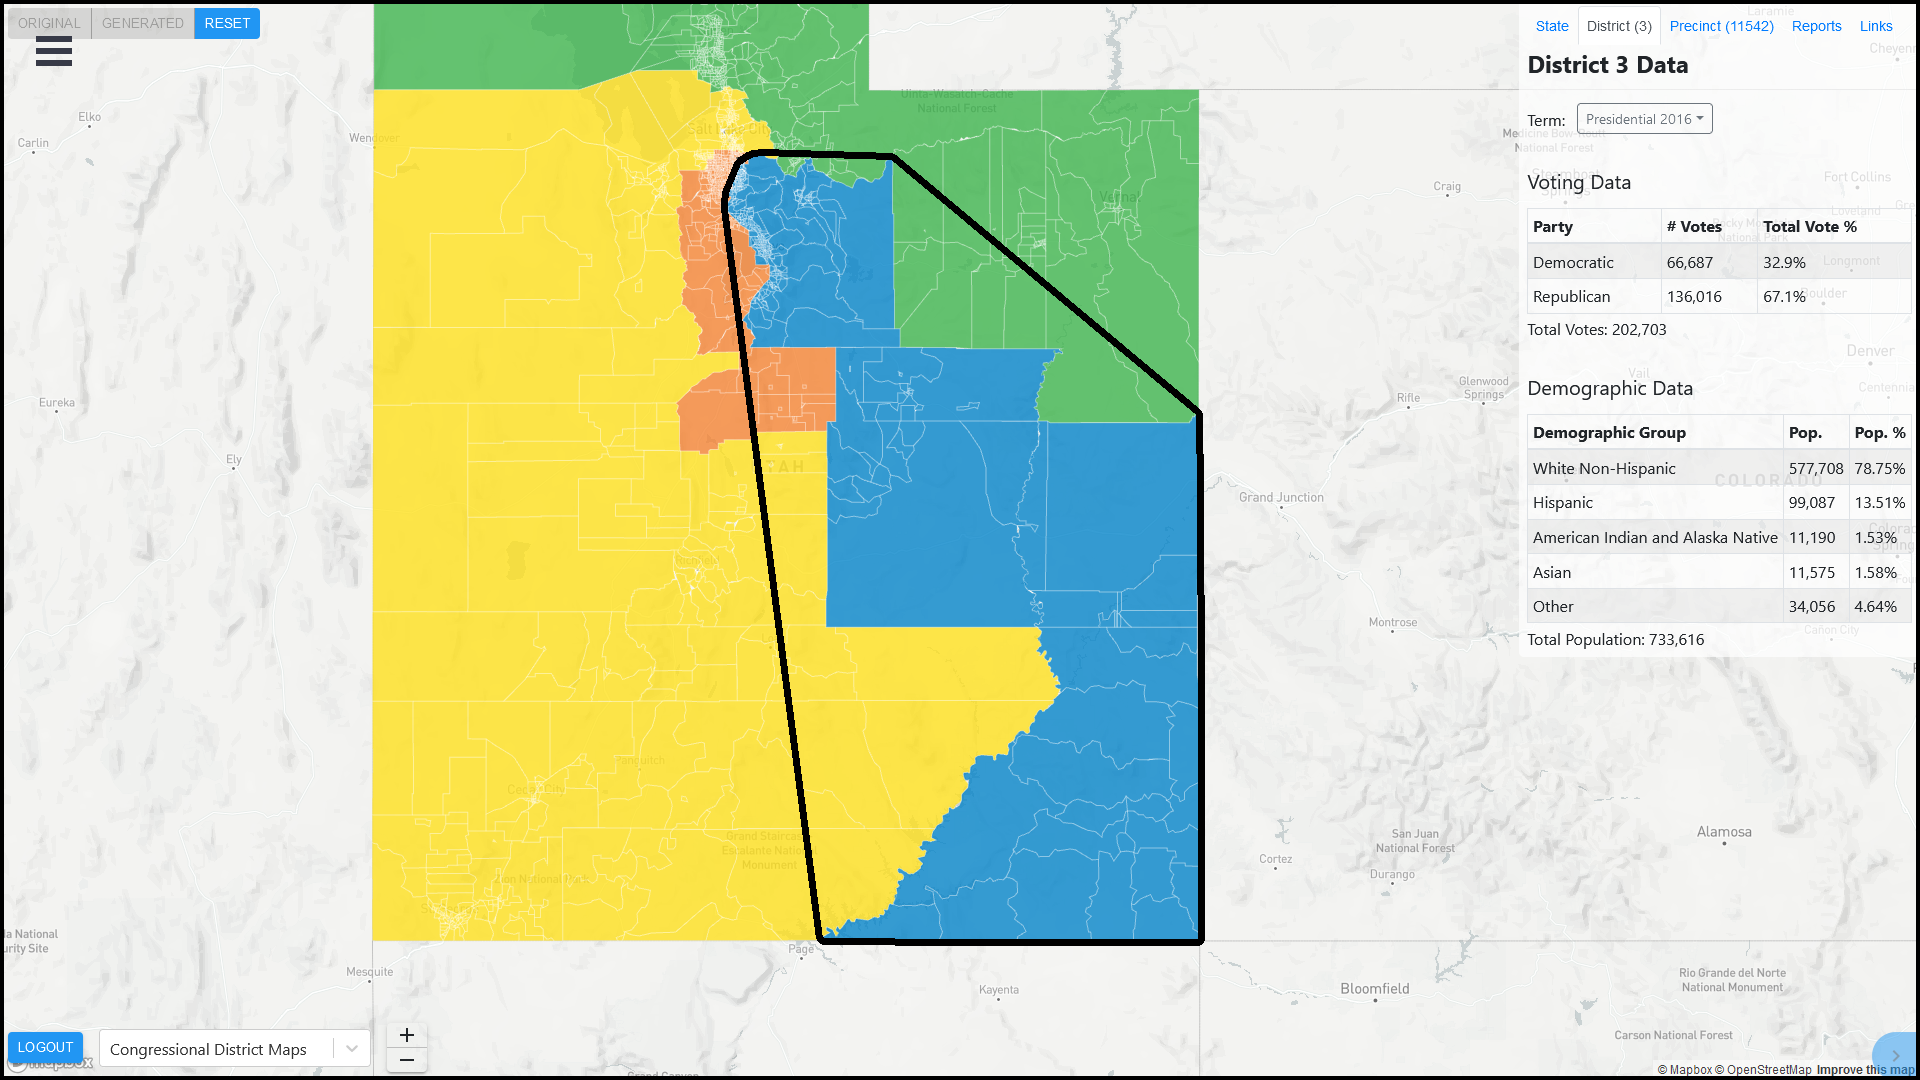
\includegraphics[width=\linewidth]{./figures/UT-03-ConvexHull.png}
	\caption{Utah District 03}
	\label{fig:ut03ch}
\end{figure}

Again, similar reasonings can be made for OR-04, OR-01, and UT-3. Even though OR-01 seems to have a "Pac-Man" shape, the convex hull simply adds the Tillamook State Forest. For the case of UT-03, it comes from the simple fact that the majority of Utah's geography is composed of deserts. Therefore, the population of the convex hull of a district would not have a major difference to the population of the district itself.

It has to be notd that many of Ohio's congressional districts have scored average or above average in regards to the Fatness score while their Polsby-Popper scores have remained low. Ohio's districts are known as the most identifiable cases of gerrymandering \cite{ohiog}. We will narrow our focus onto Ohio's 3rd and 13th congressional districts.

\begin{figure}[H]
	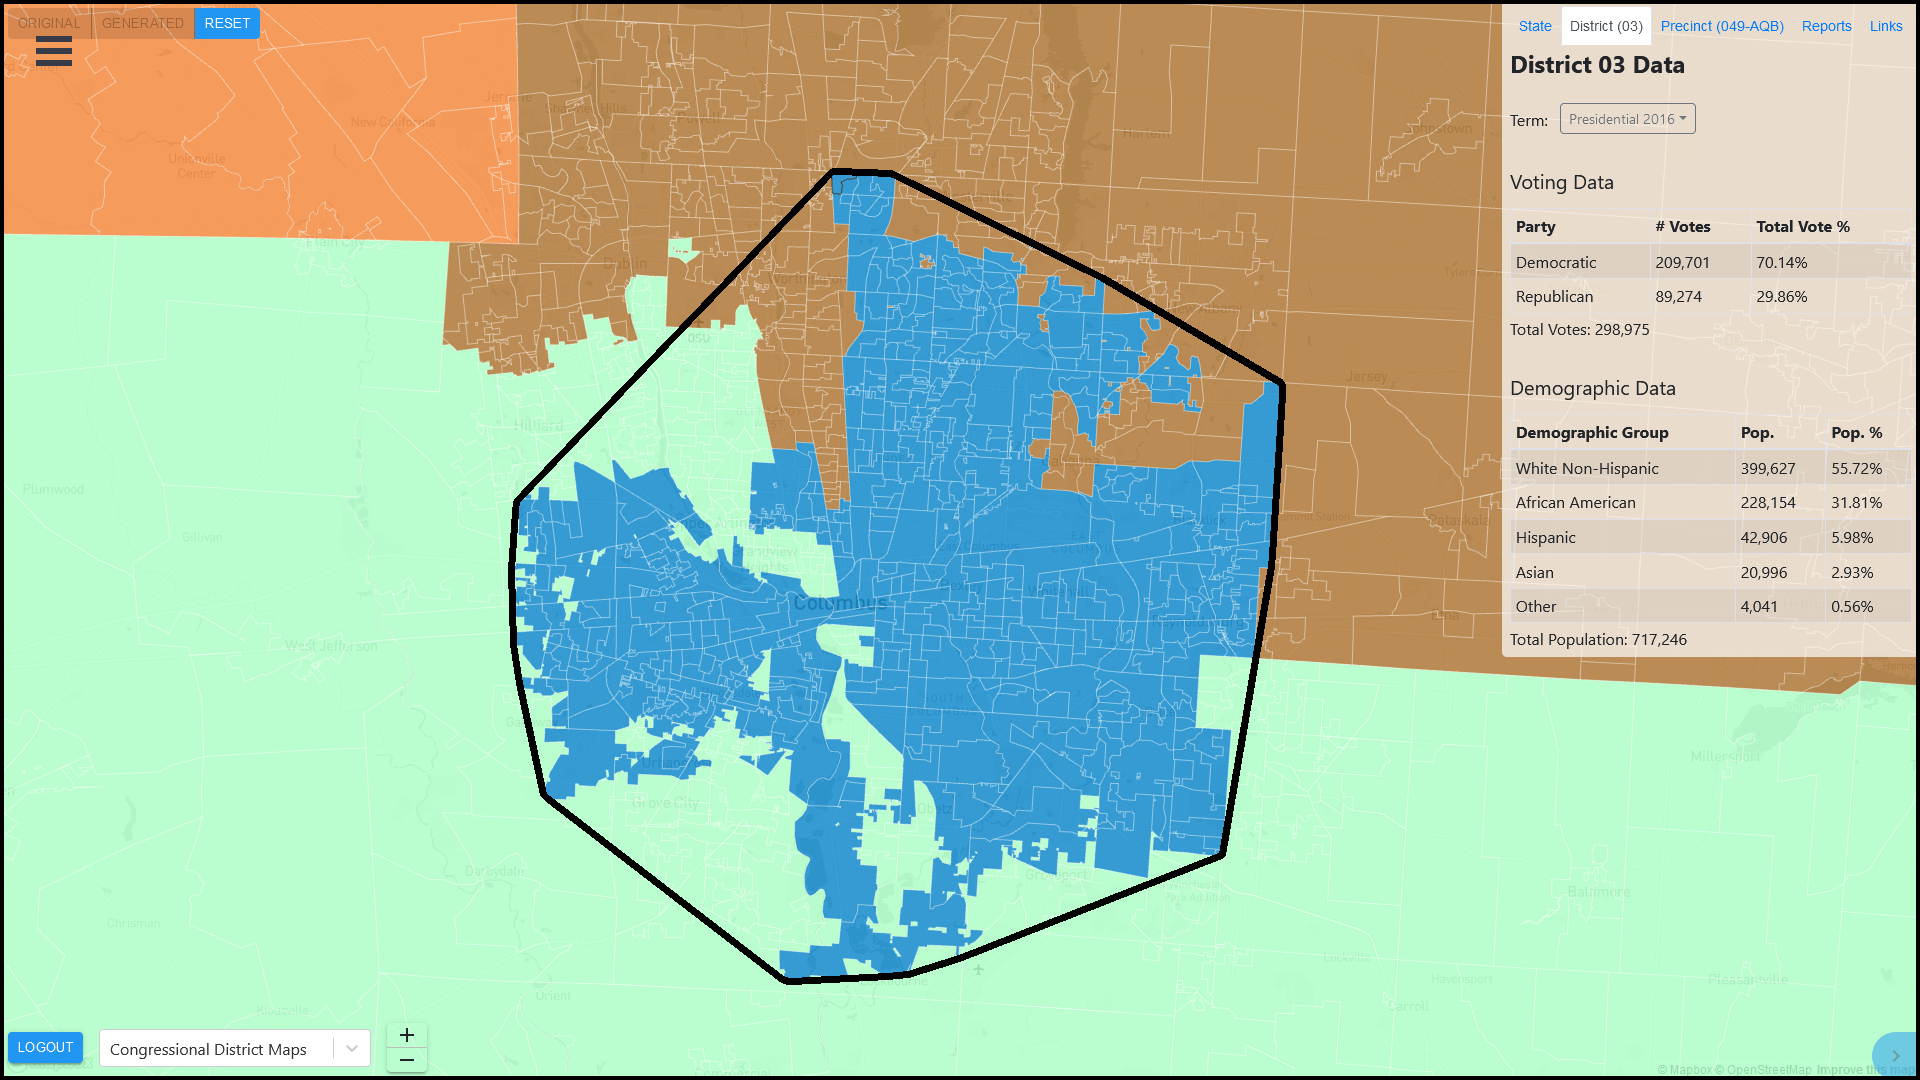
\includegraphics[width=\linewidth]{./figures/OH-03-ConvexHull.png}
	\caption{Ohio District 03}
	\label{fig:oh03ch}
\end{figure}

\begin{figure}[H]
	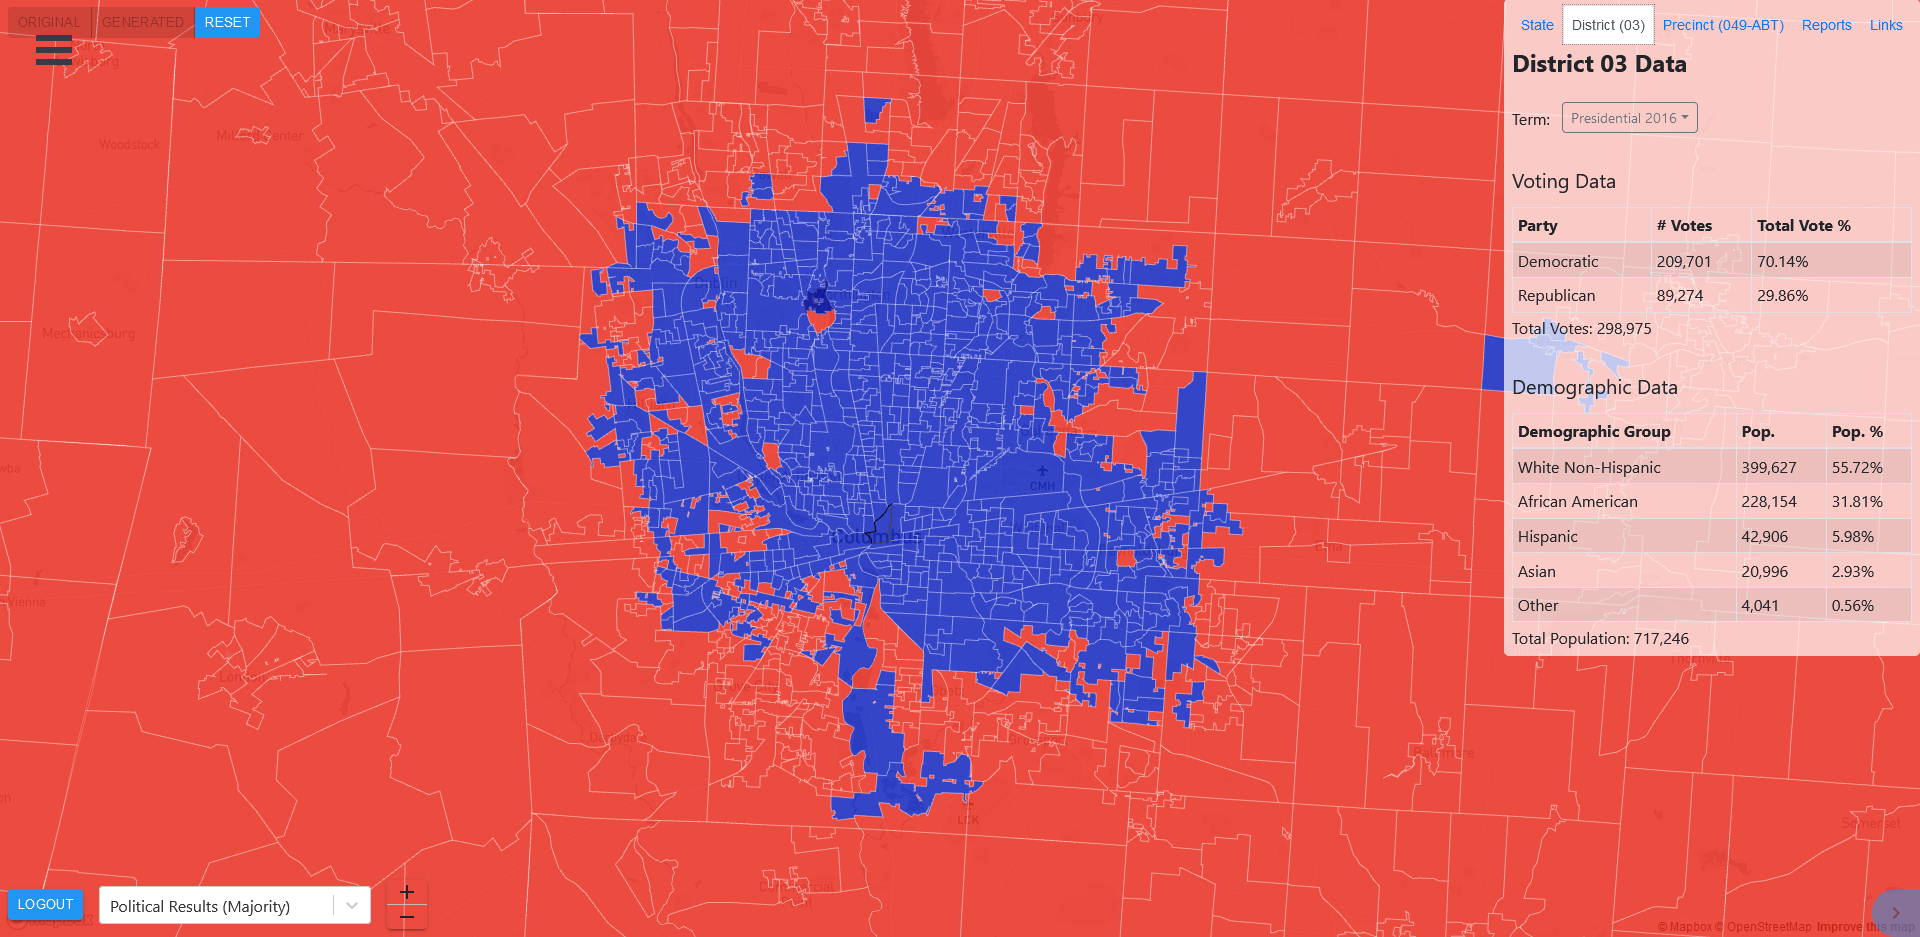
\includegraphics[width=\linewidth]{./figures/OH-03-PoliticalResults.png}
	\caption{Ohio District 03}
	\label{fig:oh03pr}
\end{figure}

In the case of OH-03, the Polsby-Popper score is low due to the meandering border that goes in and out of the city of Columbus. It extrudes and intrudes in various places, giving it a snowflake look. The average Fatness score is caused by the lack of increased population in the convex hull of the district. The area where the district seemingly avoids may just have lower population densities than the rest of Columbus. However, if we look at the political results of OH-03, we can see that the southern precincts of Columbus has a Republican majority. A case can be made that Columbus' Democratic precincts wre packed together to not dilute the Republican precints near it. A possible better redistricting would have Columbus be split or consolidated rather than the non-contiguous district that is currently implemented.

\begin{figure}[H]
	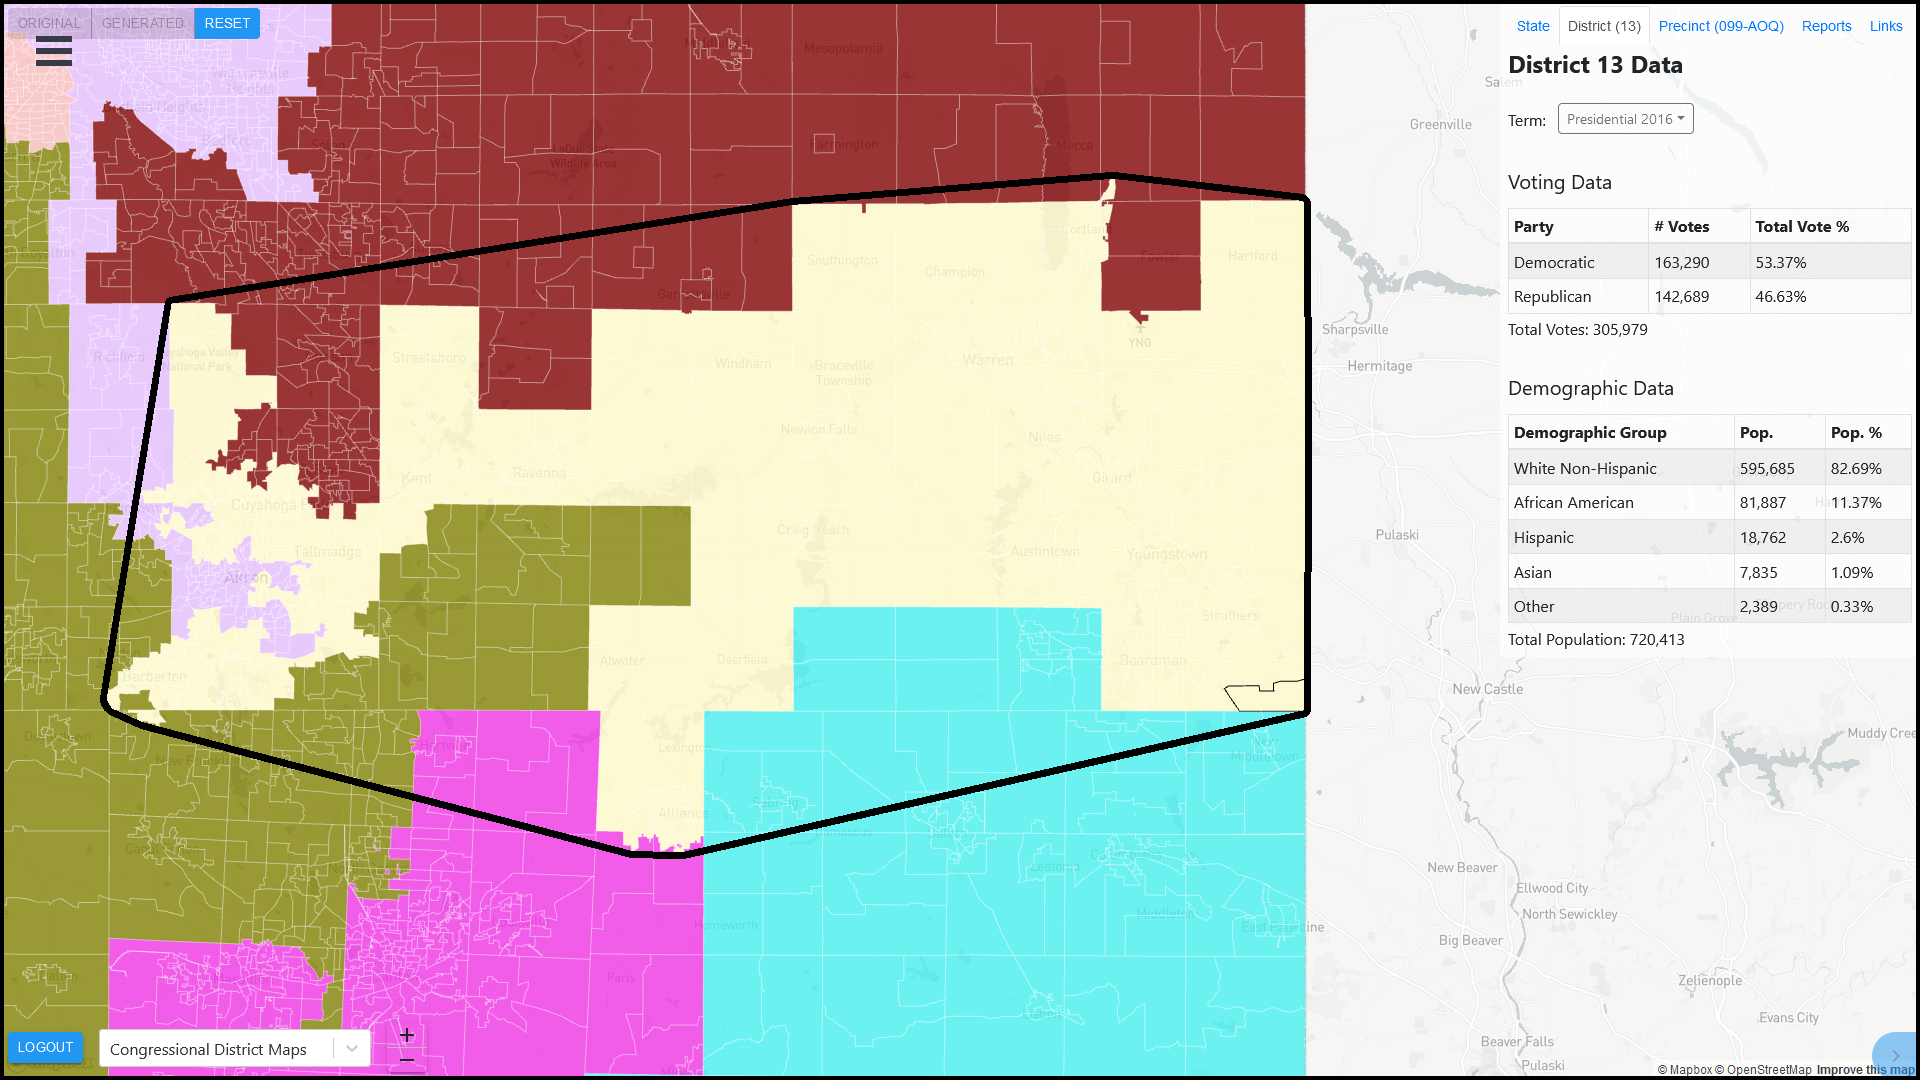
\includegraphics[width=\linewidth]{./figures/OH-13-ConvexHull.png}
	\caption{Ohio District 13}
	\label{fig:oh13ch}
\end{figure}

If we take a look at the case of OH-13, the convex hull of the district covers the entirety of the city of Akron, which the district itself avoids. The population of Akron is roughly about 200,000. The population of OH-13 is actually around 720,000 which does conveniently explain the above average score it recieves.

\section{Future Considerations}
With all of these case studies, there are quite a few things we can say about these measures and their strengths and weaknesses compared to human perception - which is supposed to be the ultimate judge.

Polsby-Popper is good at catching districts that have unnecessarily long boundaries by penalizing them. As a result, districts with long straight lines tend to be favored. Something that is both positive and negative is that it does not depend on what is going on outside of the district, which means that we cannot see if population groups are avoided, but on the other hand, districts are not graded based on their size as a dilation of district by any strictly positive constant still yields the same score. However, sometimes, the border looks straight from a distance but is not on closer inspection: this can give unnecessarily low scores, unless the border is smoothened, a less straightforward and undebatable process than it may appear. It can be stated that the main pitfall of PolsbyPopper comes from its perimeter portion of the formula. It did not take into consideration the fact that many of the districts borders follow the geography of the land or rivers. That is where the majority of the "jagged" borders of these districts come from, which in turn increases the overall perimeter of the district.

The Convex Hull Fatness improves on PolsbyPopper's faults but it leaves things to be desired. It increases the low scores given to the elongated districts like OH-10 or districts with jagged edges such as OR-01 and OR-02. However, it gives average to above average scores to many of Ohio's districtings. Specifically OH-03 and OH-13 are not considered average by the measure, but both seems to be gerrymandred due to its extrodinarly odd shape.

% Conclusion needs to be fixed
The inherent difference between both Fatness measures and Polsby-Popper is the fact that Polsby-Popper considers only the geometric portion of fatness. The Fatness improve on this by including the population requirement that all districts in a state must be of equal population. The Fatness measures undoubtly is a more accurate measure than Polsby-Popper's for many elongated and jagged districts. 
However, Fatness introduces questionable scores to others, mainly the districts of Ohio. Furthermore, it is to be noted that our measures were run on nine of the fifty total states. We had chosen these states as a representative sample of congressional districtings across the country. We could have added in more states, but it would seem redundant with the many districts we already have.

\printbibliography

\end{document}